\documentclass[12pt, a4paper]{book}
\usepackage[ascii]{inputenc}
\usepackage[left=2cm,right=2cm,top=2cm,bottom=4cm]{geometry}
\usepackage[protrusion=true,expansion=true]{microtype}

\usepackage{amsmath}
\usepackage{amsfonts}
\usepackage{amssymb}
\usepackage{tikz, pgfplots}
\usetikzlibrary{intersections}
\usetikzlibrary{decorations.pathmorphing}
\usepackage{kpfonts}
\usepackage{dsfont}
\pgfplotsset{compat=1.13}
\usepackage{emptypage}

\DeclareMathOperator{\N}{\mathbb{N}}
\DeclareMathOperator{\Q}{\mathbb{Q}}
\DeclareMathOperator{\Z}{\mathbb{Z}}
\DeclareMathOperator{\R}{\mathbb{R}}
\DeclareMathOperator{\C}{\mathbb{C}}
\DeclareMathOperator{\F}{\mathbb{F}}
\DeclareMathOperator{\ch}{ch}
\DeclareMathOperator{\KG}{KG}
\DeclareMathOperator{\SG}{SG}
\DeclareMathOperator{\ex}{ex}

\usepackage{graphicx}
\usepackage{enumitem}
\setenumerate{}

%
% Some tikz macros useful for graph theory
\tikzset{% 
    vtx/.style={inner sep=2pt,circle,fill=black}
}

%-----------------------------------------------------------------------------------------------------------------
% Some fancy macros // May eventually move these into separate files or something and merge when building template
\renewcommand{\d}[1]{\ensuremath{\operatorname{d}\!{#1}}} % dx macro for integrals
\newcommand{\hess}[1]{\ensuremath{\operatorname{H}\!{#1}}} % Hessian
\newcommand{\diff}[1]{\ensuremath{\operatorname{D}\!{#1}}} % Jacobian
\newcommand{\inner}[2]{\left\langle #1, #2 \right\rangle} % inner product
\newcommand{\norm}[1]{\left\lVert#1\right\rVert} % norm
\newcommand{\cpl}[1]{\overline{#1}} % complement
\renewcommand{\v}[1]{\mathbf{#1}} % vector
\newenvironment{amatrix}[1]{% augumented matrix - make sure to have # columns less than required amount
  \left(\begin{array}{@{}*{#1}{c}|c@{}}
}{%
  \end{array}\right)
}
%-----------------------------------------------------------------------------------------------------------------
% Define theorem environments, along with a custom proof environment
\usepackage[thref, thmmarks,amsmath]{ntheorem}
\newcommand{\itref}[1]{\textit{\thref{#1}}}

\newtheorem{theorem}{Thm.}[section]
\newtheorem{conjecture}[theorem]{Con.}
\newtheorem{lemma}[theorem]{Lemma}
\newtheorem{definition}[theorem]{Def'n.}
\newtheorem{corollary}[theorem]{Cor.}
\newtheorem{proposition}[theorem]{Prop.}

\theorembodyfont{\upshape}
\newtheorem{remark}[theorem]{Rmk.}
\newtheorem{exercise}[theorem]{Exc.}
\newtheorem{example}[theorem]{Ex.}
\theoremseparator{}
\theoremindent0.0cm
\theoremstyle{nonumberplain}
\theoremheaderfont{\scshape}
\theoremsymbol{$\square$}
\newtheorem{proof}{Proof}

%-----------------------------------------------------------------------------------------------------------------
% Define Document Variables
\newcommand{\assignmentname}{Course Notes}
\newcommand{\classname}{Graph Theory}
\newcommand{\semester}{BSM Fall 2018}

% Define a title page for the document
%----------------------------------------------------------------------------------------------------------------------
% Define headings for each page
\usepackage{fancyheadings}
\pagestyle{fancy}
\lhead{Alex Rutar\\arutar@uwaterloo.ca}
\rhead{\classname: \assignmentname\\\semester}
\cfoot{\thepage}
\setlength{\headheight}{50pt}
%----------------------------------------------------------------------------------------------------------------------
\begin{document}
\pagenumbering{roman}
\begin{titlepage}
    \centering
    \vspace{5cm}
    {\huge\textbf{\assignmentname}\par} % Assignment Name
    \vspace{2cm}
    {\Large\textbf{\classname}\par} % Class
    \vspace{3cm}
    {\Large\textit{Alex Rutar}\par}

    \vfill

% Bottom of the page
    {\large \semester \par} % Due Date
\end{titlepage}
%----------------------------------------------------------------------------------------------------------------------
\pagenumbering{roman}
\tableofcontents
\pagenumbering{arabic}
\chapter{Basic Structure of Graphs}
\section{A Brief Introduction}
\subsection{Basic Definitions}
\begin{definition}
    A \textbf{simple graph} $G=(V,E)$ consists of a vertex set $V$ and edge set $E$ where $E\subseteq\binom{V}{2}$.
\end{definition}
Note that we write $\binom{V}{2}$ instead of $V\times V$ to make it clear that we cannot have loops and multiple edges.
If the graph is undirected, edges are unordered pairs $\{v_1,v_2\}$ of vertices; we write $(v_1,v_2)$ for directed edges.
\begin{definition}
    Two graphs $F$ and $G$ are \textbf{isomorphic} if there exists a bijective mapping $f:V(F)\to V(G)$ such that for every $a,b\in V(F)$: $\{a,b\}\in E(F)\Leftrightarrow \{f(a),f(b)\}\in E(G)$.
\end{definition}
\begin{definition}
    The \textbf{degree} of a vertex $v\in V(G)$ is the number of edges having $v$ as an endpoint.
    We denote this number by $d(v)$, and $\Delta(G)$ to denote the maximal degree in $G$, and $\delta(G)$ to denote the minimal degree in $G$.
\end{definition}
\begin{definition}
    The \textbf{vertex neighbourhood} of a graph $U$ is denoted by $N(U):=\{v\in V(G):\exists u\in U\text{ s.t. }\{v,u\}\in E(G)\}$.
\end{definition}
\begin{definition}
    A \textbf{path} is a sequence $v_1e_1v_2e_2\ldots v_ie_iv_{i+1}\ldots e_jv_{j+1}$ where each $v_i\in V(G)$ and $e_i=\{v_i,v_{i+1}\}\in E(G)$ where all $v_i$'s are different.
    A \textbf{cycle} is a path in which $v_1=v_{j+1}$.
\end{definition}
\begin{definition}
    The \textbf{complementary graph} of $G=(V,E)$ is $\overline{G}=\left(V,\binom{V}{2}\setminus E\right)$.
\end{definition}
\begin{definition}
    A graph $G$ is called \textbf{connected} if for every $u,v\in V(G)$ there exists a path between $u$ and $v$.
\end{definition}
\begin{definition}
    A connected graph that becomes disconnected with the removal of any edge is called a \textbf{tree}.
    Equivalently, a \textbf{tree} is a graph which is connected and contains no cycle.
\end{definition}
\begin{proposition}
    Any tree on at least two vertices contains at least two vertices of degree 1 (``leaves'').
\end{proposition}
\begin{proof}
    Consider a path of maximal length.
    We claim that both endpoints of $P$ have degree one.
    Suppose for contradiction that an endpoint has greater than one.
    Then the endpoint has another neighbour on the path (in which case we have a cycle), or a unique neighbour (in which case the path is not maximal), a contradiction in either case.
\end{proof}
\begin{proposition}
    A tree on $n$ vertices always has $n-1$ edges.
\end{proposition}
\begin{proof}
    Delete the edges one by one.
    Each time, the number of connected components increases by one.
    After deleting all edges, we have $n$ components, at the beginning, we have one, so we deleted $n-1$ edges.
\end{proof}
\subsection{Pr\"ufer Codes}
We now have an interesting question: how many different trees can be given on $n$ labelled vertices?
To investigate this, we consider the Pr{\"u}fer code. Delete the smallest labelled degree one vertex and write up its unique neighbour's label.
Continue doing this until only one point remains.
The obtained sequences of labels is the Pr\"ufer code.

Properties:
\begin{itemize}[nolistsep]
    \item The length is $n-1$
    \item The last digit must be $n$
\end{itemize}
\begin{theorem}[Cayley]
    The number of different trees on $n$ labelled vertices is $n^{n-2}$.
\end{theorem}
\begin{proof}
    We will show that sequences $x\in\{1,2,\ldots,n\}^{n-1}$ with $x_{n-1}=n$ are in bijective correspondence with the trees on $n$ labelled vertices.
    First, given $a_1a_2\ldots a_{n-2}a_{n-1}$ with $a_{n-1}=n$ we want to decode it.
    Let $b_1,b_2,\ldots,b_{n-1}$ be the sequence of labels of vertices deleted in the order of the indices.
    If we ``decode'' $b_1b_2\ldots b_{n-1}$, we know the tree, since we have the $n-1$ edges $\{a_i,b_i\}$.
    \begin{enumerate}
        \item $b_1:=\min\{k\in\{1,2,\ldots,n\}:k\notin \{a_1,\ldots,a_{n-1}\}\}$
        \item $b_2:=\min\{k\in\{1,2,\ldots,n\}:k\notin \{b_1,a_2,\ldots,a_{n-1}\}\}$
        \item[$(*)$] \fbox{$b_i:=\min\{k\in\{1,2,\ldots,n\}:k\notin \{b_1,\ldots,b_{i-1},a_i,\ldots,a_{n-1}\}\}$}
    \end{enumerate}
    We show that taking any sequence $a_1a_2\ldots a_{n-1}$ with $a_{n-1}=n$ and applying $(*)$ to obtain $b_1,\ldots,b_{n-1}$, the graph we obtain on vertices $1,\ldots,n$ with the $n-1$ edges $\{a_i,b_i\}$ (1) is a tree, and (2) has Pr\"ufer code is just $a_1a_2\ldots a_{n-1}$.

    Note that $(*)$ implies that $\{b_1,b_2,\ldots,b_{n-1},a_{n-1}\}=\{1,2,\ldots,n\}$.
    Define graphs $T_i$ for $i=n-1,n-2,\ldots,2,1$ on the graph spanned by the edges $\{a_{n-1},b_{n-1}\},\{a_{n-2},b_{n-2}\},\ldots,\{a_i,b_i\}$.
    It suffices to prove that $T_i$ is a tree for every $i$ and $b_i$ is its smallest labelled degree 1 vertex.

    We do this by induction.
    Clearly, it is true for $i=n-1$.
    Once it is true for $i=n-1,\ldots,j+1$, we prove this for $i=j$.
    We know that $T_{j+1}$ is a tree, and we wish to add the edge $\{b_j,a_j\}$.
    Thus $b_j\notin V(T_{j+1})=\{b_{j+1},b_{j+2},\ldots,b_{n-1},a_{n-1}\}$ so $b_j$ is indeed degree one; $a_j\in V(T_{j+1})$ and $T_j$ is a tree.
    If $b_j$ was not the smallest degree 1 vertex, then there exists some $k>j$ such that $b_k<b_j$ and $b_k$ has degree one in $T_j$.
    But then $b_k\notin\{b_1,\ldots,b_{j-1},a_j,\ldots,a_{n-1}\}$ so $(*)$ would have chosen it in place of $b_j$, a contradiction.

\end{proof}
Here's an illustration of a particular tree along with the corresponding Pr\"ufer code.:
\begin{center}
    \begin{tikzpicture}[lvtx/.style={inner sep=3pt,circle,draw=black,thick}]
        \node[lvtx] (1) at (0,0){\tiny 1};
        \node[lvtx] (2) at (0,1){\tiny 3};
        \node[lvtx] (3) at (1,1){\tiny 2};
        \node[lvtx] (4) at (1,2){\tiny 6};
        \node[lvtx] (5) at (2,0){\tiny 5};
        \node[lvtx] (6) at (2,2){\tiny 7};
        \node[lvtx] (7) at (2,3){\tiny 4};

        \path[]
            (1) edge[thick] (3)
            (3) edge[thick] (2)
            (3) edge[thick] (5)
            (3) edge[thick] (4)
            (4) edge[thick] (6)
            (4) edge[thick] (7);
        \node (l) at (5,1.5){$\Longrightarrow\qquad(2,2,6,2,6,7)$};
    \end{tikzpicture}
\end{center}
We then have
\begin{align*}
    a_1&=2 & b_1 &= \min\{k\in[7],k\notin\{2,2,6,2,6,7\}\}=1\\
    a_2&=2 & b_2 &= \min\{k\in[7],k\notin\{1,2,6,2,6,7\}\}=3\\
    a_3&=6 & b_3 &= \min\{k\in[7],k\notin\{1,3,6,2,6,7\}\}=4\\
    a_4&=2 & b_4 &= \min\{k\in[7],k\notin\{1,3,4,2,6,7\}\}=5\\
    a_5&=6 & b_5 &= \min\{k\in[7],k\notin\{1,3,4,5,6,7\}\}=2\\
    a_6&=7 & b_6 &= \min\{k\in[7],k\notin\{1,3,4,5,2,7\}\}=6
\end{align*}
so that the edges are given by $E(G)=\{ \{1,2\},\{3,2\},\{4,6\},\{5,2\},\{2,6\},\{6,7\}\}$.


\section{Paths, Circuits, and Cycles}
\subsection{Eulerian Circuits}
\begin{definition}
    An \textbf{Eulerian circuit} is a closed walk in a graph that contains every edge exactly once.
    An \textbf{Eulerian path} is a walk containing every edge exactly once and not (necessarily) ending at the same vertex.
\end{definition}
Note that we do allow multiple edges between vertices.
We also assume that our graph is connected.
\begin{theorem}[Euler]
    A graph contains an Eulerian circuit if and only if every vertex has even degree.
\end{theorem}
\begin{corollary}
    A graph contains an Eulerian path if and only if all but two vertices have even degree.
\end{corollary}
In both cases, necessity is obvious: every time a path arrives at a vertex, it adds two to the degree since there is a unique edge in and out from the vertex.
Thus for the corollary the only odd vertices can be the endpoints, and for the theorem, there are no endpoints in the path.
\begin{proof}[cor.]
    To see the corollary, first add an edge connecting the two odd degree vertices.
    Then by the theorem, we have an Eulerian circit walk through it so that the added edge is the last one traversed.
    Delete it, and the remaining part of the walk gives our Eulerian path
\end{proof}
\begin{proof}[thm.]
    We can now prove the theorem.
    Consider a maximal walk $P$ on $G$ that does not repeat edges.
    Because of the evenness of all degrees, it must be closed.
    If every edge is contained, it is an Eulerian circuit and we are done.
    If there exists some $e\in E(G)$ that is not in the walk, then by connectedness, there must be a path from a vertex in the walk to an endpoint of $e$.
    Considering a shortest such path (perhaps containing 0 edges), all edges on it are unused so far.
    Now take the starting point of this path on our walk, go through the closed path on our walk, go through the closed walk we have starting here and thus contine on the said path and include $e$, a contradiction.
\end{proof}
\subsection{Hamiltonian Cycles}
\begin{definition}
    A \textbf{Hamiltonian cycle} in a graph is a cycle containing every vertex exactly once.
    A \textbf{Hamiltonian path} is a path that contains every vertex exactly once.
\end{definition}
\subsection{Necessary Conditions}
\begin{proposition}
    If $G$ contains a Hamiltonian cycle, then after deleting any $k$ of its vertices, the remaining graph cannot have more than $k$ components.
    Similarly, if $G$ contains a Hamiltonian path, then deleting any $k$ of it vertices yields a graph with at most $k+1$ components.
\end{proposition}
\begin{proof}
    This can be easily proven by induction.
\end{proof}
Here is a graph for which this condition holds, but does not have a Hamiltonian cycle.
\begin{center}
    \begin{tikzpicture}[
        vtx/.style={circle,radius=0.5pt,fill=black,inner sep=2pt},
        edge/.style={thick},
        scale=0.5
        ]
        \node[vtx, fill=red] (1a) at (18:2cm){};
        \node[vtx, fill=red] (2a) at (90:2cm){};
        \node[vtx] (3a) at (162:2cm){};
        \node[vtx] (4a) at (234:2cm){};
        \node[vtx] (5a) at (306:2cm){};

        \node[vtx] (1b) at (18:4cm){};
        \node[vtx] (2b) at (90:4cm){};
        \node[vtx] (3b) at (162:4cm){};
        \node[vtx] (4b) at (234:4cm){};
        \node[vtx] (5b) at (306:4cm){};

        \draw[edge] (1b) -- (2b) -- (3b) -- (4b) -- (5b) -- (1b);
        \draw[edge] (1a) -- (1b);
        \draw[edge] (2a) -- (2b);
        \draw[edge] (3a) -- (3b);
        \draw[edge] (4a) -- (4b);
        \draw[edge] (5a) -- (5b);
        \draw[edge] (1a) -- (3a) -- (5a) -- (2a) -- (4a) -- (1a);
    \end{tikzpicture}
\end{center}
The condition holds: delete $k=l_1+l_2$ vertices, where $l_1$ is in the ``outer cycle'' and $l_2$ is in the ``inner cycle''.
(Above, $l_1=0$ and $l_2=2$.)
Then the outer cycle may not fall apart into more than $l_1$ components, the inner cycle may not fall apart into more than $l_2$ component, so if $l_1,l_2>0$, then there are at most $l_1+l_2$ components.
If $l_1$ or $l_2$ is $0$, then the graph remains connected.

Furthermore, there does not exist a Hamiltonian cycle.
Suppose such a cycle exists, then it is a cycle containing 10 edges.
Colour the alternating edges red and blue.
Thus every vertex is adjacent to a red edge and a blue edge.
Colour the remaining 5 edges white, so every vertex will be the end vertex of exactly 1 white edge.
However, such an edge-coloring is impossible.

Up to isomorphism, the outer edges must be coloured with two of colour 1, two of colour 2, and one of colour 3.
We then fill in the interior edges as required, until the inner cycle, in which we are forced to draw the following edges, yielding our contradiction.
\begin{center}
    \begin{tikzpicture}[
        scale=0.5,
        vtx/.style={circle,radius=0.5pt,fill=black,inner sep=2pt},
        edge/.style={thick}
        ]
        \node[vtx] (1a) at (18:2cm){};
        \node[vtx] (2a) at (90:2cm){};
        \node[vtx] (3a) at (162:2cm){};
        \node[vtx] (4a) at (234:2cm){};
        \node[vtx] (5a) at (306:2cm){};

        \node[vtx] (1b) at (18:4cm){};
        \node[vtx] (2b) at (90:4cm){};
        \node[vtx] (3b) at (162:4cm){};
        \node[vtx] (4b) at (234:4cm){};
        \node[vtx] (5b) at (306:4cm){};

        \draw[edge,draw=blue] (1b) -- (2b);
        \draw[edge,draw=red] (2b) -- (3b);
        \draw[edge,draw=blue] (3b) -- (4b);
        \draw[edge,draw=red] (4b) -- (5b);
        \draw[edge,draw=green] (5b) -- (1b);

        \draw[edge,draw=red] (1a) -- (1b);
        \draw[edge,draw=green] (2a) -- (2b);
        \draw[edge,draw=green] (3a) -- (3b);
        \draw[edge,draw=green] (4a) -- (4b);
        \draw[edge,draw=blue] (5a) -- (5b);

        \draw[edge] (1a) -- (3a);
        \draw[edge] (3a) -- (5a);
        \draw[edge] (5a) -- (2a);
        \draw[edge] (2a) -- (4a);
        \draw[edge] (4a) -- (1a);
    \end{tikzpicture}
    \qquad
    \begin{tikzpicture}[
        scale=0.5,
        vtx/.style={circle,radius=0.5pt,fill=black,inner sep=2pt},
        edge/.style={thick}
        ]
        \node[vtx] (1a) at (18:2cm){};
        \node[vtx] (2a) at (90:2cm){};
        \node[vtx] (3a) at (162:2cm){};
        \node[vtx] (4a) at (234:2cm){};
        \node[vtx] (5a) at (306:2cm){};

        \node[vtx] (1b) at (18:4cm){};
        \node[vtx] (2b) at (90:4cm){};
        \node[vtx] (3b) at (162:4cm){};
        \node[vtx] (4b) at (234:4cm){};
        \node[vtx] (5b) at (306:4cm){};

        \draw[edge,draw=blue] (1b) -- (2b);
        \draw[edge,draw=red] (2b) -- (3b);
        \draw[edge,draw=blue] (3b) -- (4b);
        \draw[edge,draw=red] (4b) -- (5b);
        \draw[edge,draw=green] (5b) -- (1b);

        \draw[edge,draw=red] (1a) -- (1b);
        \draw[edge,draw=green] (2a) -- (2b);
        \draw[edge,draw=green] (3a) -- (3b);
        \draw[edge,draw=green] (4a) -- (4b);
        \draw[edge,draw=blue] (5a) -- (5b);

        \draw[edge,draw=blue] (1a) -- (3a);
        \draw[edge,draw=red] (3a) -- (5a);
        \draw[edge,draw=red] (5a) -- (2a);
        \draw[edge] (2a) -- (4a);
        \draw[edge,draw=blue] (4a) -- (1a);
    \end{tikzpicture}
\end{center}
\subsection{Sufficient Conditions}
\begin{theorem}[Dirac, 1952]
    If $G$ is a graph on $n$ vertices, with every degree being at least $\frac{n}{2}$, then $G$ contains a Hamiltonian cycle.
\end{theorem}
\begin{proof}
    Follows from Ore's Theorem.
\end{proof}
This bound is tight: for every graph on $n$ vertices, $f(n)\geq n/2$ is the minimal requirement since the graph composed of two disconnected components $K_{n/2}$ has degree $n/2-1$ everywhere but does not have a Hamiltonian cycle.
As a fun fact, this is not Paul Dirac, but rather Gabriel Andrew Dirac (Paul Dirac's stepson).
\begin{theorem}[Ore, 1960]
    If $G$ is a graph on $n$ vertices such that for every nonadjacent pair of vertices $u,v\in V(G)$, $d(u)+d(v)\geq n$ is satisfied, then $H$ contains a Hamiltonian cycle.
\end{theorem}
\begin{proof}
    Assume for contradiction we have $G_0$ satisfying the condition but does not have a Hamiltonian cycle.
    Saturate $G_0$ go obtain $G$: if two vertices are non-adjacent and connecting them does not create a Hamiltonian cycle, then connect them.
    This new graph is still a counterexample since whenever we increase the degree of some vertices, they are no longer non-adjacent.
    Do this maximally, so that the addition of any edge would create a Hamiltonian cycle and $G$ still satisfies Ore's condition.

    Now, if $a,b\in V(G)$ are non-adjacent in $G$, then there exists a Hamiltonian path starting at $a$ and ending at $b$ (since adding $\{a,b\}$ would create a Hamiltonian cycle).
    Consider such a Hamiltonian path $(x_1,x_2,\ldots,x_n)$.
    \begin{center}
        \begin{tikzpicture}
            \node[circle,inner sep=2pt,fill=black,label=below:{$a=x_1$}] (x1) at (0,0){};
            \node[circle,inner sep=2pt,fill=black,label=above:{$x_2$}] (x2) at (1,0){};
            \node[circle,inner sep=2pt,fill=black,label=above:{$x_3$}] (x3) at (2,0){};
            \node[circle,inner sep=2pt,fill=black,label=above:{$x_{i-1}$}] (xim1) at (5,0){};
            \node[circle,inner sep=2pt,fill=black,label=above:{$x_i$}] (xi) at (6,0){};
            \node[circle,inner sep=2pt,fill=black,label=above:{$x_{i+1}$}] (xip1) at (7,0){};
            \node[circle,inner sep=2pt,fill=black,label=above:{$x_{n-1}$}] (xnm1) at (10,0){};
            \node[circle,inner sep=2pt,fill=black,label=above:{$x_{n}=b$}] (xn) at (11,0){};

            \node[inner sep=0pt] (a) at (3,0){};
            \node[inner sep=0pt] (b) at (4,0){};
            \node[inner sep=0pt] (c) at (8,0){};
            \node[inner sep=0pt] (d) at (9,0){};

            \draw (x1) -- (x2) -- (x3) -- (a);
            \draw[dotted] (a) -- (b);
            \draw (b) -- (xim1) -- (xi) -- (xip1) -- (c);
            \draw[dotted] (c) -- (d);
            \draw (d) -- (xnm1) -- (xn);

            \draw plot [smooth, tension=1.4] coordinates { (x1) (3,1) (xi)};
            \draw [dashed] plot [smooth, tension=1.4] coordinates { (xim1) (8,-1) (xn)};
            \node (X) at (8,-1){\large $\times$};
        \end{tikzpicture}
    \end{center}
    Observe that if $\{a,x_i\}\in E(G)$, then $\{a,x_{i-1}\}\notin E(G)$ or we would have a Hamiltonian cycle given by $(a,x_i,x_{i+1},\ldots,b,x_{i-1},x_{i-2},\ldots,a)$.
    This implies that $d(b)\leq n-1-d(a)$: for each neighbour of $a$, there is a distinct non-neighbour of $b$.
    But this is a contradiction since $d(a)+d(b)\leq n-1$ while $\{a,b\}\notin E(G)$ and $G$ does not satisfy the condition.
\end{proof}
\begin{theorem}[P\'osa, 1962]
    Let $G$ be a graph on $n$ vertiecs with degrees $d_1\leq d_2\leq\cdots\leq d_n$.
    Then for every $k<n/2$, we have $d_k\geq k+1$, then $G$ contains a Hamiltonian cycle.
\end{theorem}
\begin{proof}
    Again, follows from Chv\'atal's Theorem below.
\end{proof}
\begin{theorem}[Chv\'atal, 1972]
    \hfill
    \begin{enumerate}[nolistsep, label=(\roman*)]
        \item Let $G$ be a graph on $n$ vertices with degrees $d_1\leq d_2\leq\cdots\leq d_n$.
            Assume that whenever for some $k<n/2$, if we have $d_k\leq k$, $d_{n-k}\geq n-k$.
            Then $G$ contains a Hamiltonian cycle.
        \item Assume that the number $d_1'\leq d_2'\leq\cdots d_n'$ do not satisfy the implication.
            Then there exists a graph $G$ with degrees $d_1\leq d_2\leq\cdots\leq d_n$ such that $d_i\geq d_i'$ and $G$ has no Hamiltonian cycle.
    \end{enumerate}
\end{theorem}
\begin{proof}
    \begin{enumerate}[label=(\roman*)]
        \item Assume that the statement is false, consider a counterexample $G_0$, and saturate it to obtain $G$.
            This works: adding edges only increases the degrees of the vertices, and thus the values of $d_k$ and $d_{n-k}$, so the condition still holds.
            Now, from Ore's proof, we know that for every $a,b\in V(G)$ that are non-adjacent, there exists a Hamiltonian path from $a$ to $b$ and $d(a)+d(b)\leq n-1$.
            Consider an $a,b\in V(G)$, $\{a,b\}\notin E(G)$ pair for which $d(a)+d(b)$ is maximal
            \begin{center}
                \begin{tikzpicture}
                    \node[circle,inner sep=2pt,fill=black,label=below:{$a=x_1$}] (x1) at (0,0){};
                    \node[circle,inner sep=2pt,fill=black,label=above:{$x_2$}] (x2) at (1,0){};
                    \node[circle,inner sep=2pt,fill=black,label=above:{$x_3$}] (x3) at (2,0){};
                    \node[circle,inner sep=2pt,fill=black,label=above:{$x_{i-1}$}] (xim1) at (5,0){};
                    \node[circle,inner sep=2pt,fill=black,label=above:{$x_i$}] (xi) at (6,0){};
                    \node[circle,inner sep=2pt,fill=black,label=above:{$x_{i+1}$}] (xip1) at (7,0){};
                    \node[circle,inner sep=2pt,fill=black,label=above:{$x_{n-1}$}] (xnm1) at (10,0){};
                    \node[circle,inner sep=2pt,fill=black,label=above:{$x_{n}=b$}] (xn) at (11,0){};

                    \node[inner sep=0pt] (a) at (3,0){};
                    \node[inner sep=0pt] (b) at (4,0){};
                    \node[inner sep=0pt] (c) at (8,0){};
                    \node[inner sep=0pt] (d) at (9,0){};

                    \draw (x1) -- (x2) -- (x3) -- (a);
                    \draw[dotted] (a) -- (b);
                    \draw (b) -- (xim1) -- (xi) -- (xip1) -- (c);
                    \draw[dotted] (c) -- (d);
                    \draw (d) -- (xnm1) -- (xn);

                    \draw plot [smooth, tension=1.4] coordinates { (x1) (3,1) (xi)};
                    \draw [dashed] plot [smooth, tension=1.4] coordinates { (xim1) (8,-1) (xn)};
                    \node (X) at (8,-1){\large $\times$};
                \end{tikzpicture}
            \end{center}
            We may assume $d(a)\leq d(b)$ so that $d(a)\leq\frac{n-1}{2}<\frac{n}{2}$.
            For notation, fix $h=d(a)$; we claim that $d_h\leq h<\frac{n}{2}$.
            We show $d_h\leq h$.
            
            Now consider the vertices $x$ which are not neighbours of $b$.
            Since $\{x,b\}$ is a non-adjacent pair of $b$ which is not maximal, we must have $d(x)\leq d(a)=h$.
            Furthermore, from the Ore proof argument, we know that the number of non-neighbours of $b$ is at least as large as $d(a)=h$, so there are at least $h$ vertices with $d(x)\leq h$.
            Thus $d_h\leq h$ and we have our claim.

            Thus by our condition, $d_{n-h}\geq n-h$, so there exist $h+1$ vertices with degree at least $n-h$.
            Since $d(a)=h$, there exists some non-neighbour $y$ of $a$ with $d(y)\geq n-h$.
            But then $\{a,y\}$ is a non-adjacent pair with $d(a)+d(y)\geq h+n-h=n>d(a)+d(b)$, a contradiction to the choice of $\{a,b\}$.
        \item Assume $d_1'\leq\cdots\leq d_n'$ violates our condition.
            Then we have $k$ so that $d'_k\leq k<n/2$ and $d'_{n-k}\leq n-k-1$.
            Fix such a $k$, then
            \[d_1'\leq d_2'\leq\cdots\leq d_k'\leq k\]
            \[d_{k+1}'\leq d_{k+2}'\leq\cdots\leq d_n'\leq n-k-1\]
            and clearly, $d_{n-k+1}'\leq\cdots\leq d_n'\leq n-1$.
            Set $d_1=d_2=\cdots=d_k:= k$, $d_{k+1},d_{k+2}=\cdots=d_{n-k}:=n-k-1$ and $d_{n-k+1}=\cdots=d_n:=n-1$.
            Thus it is enough to show a graph with these degrees and no Hamiltonian cycle.
            Here is such a graph:
            \begin{center}
                \begin{tikzpicture}
                    \draw (0,0) ellipse (1cm and 2cm) node{$k$};
                    \draw (3,0) ellipse (1cm and 2cm) node{$k$};
                    \draw (6,0) ellipse (1cm and 2cm) node{$n-2k$};
                    \draw[dashed] (4.5,0) ellipse (3cm and 3cm);
                    \draw[dashed] (1.5,0) ellipse (3cm and 3cm);
                    \node[below] (a) at (1.5,-3){$K_{k,k}$};
                    \node[below] (b) at (4.5,-3){$K_{n-k}$};
                \end{tikzpicture}
            \end{center}
            It can be verified that the degrees in the first compoent are $k$, second are $n-1$ and third are $n-k-1$.
            Furthermore, the graph has no Hamiltonian cycle.
            Remove the $k$ vertices of degree $N-1$, and we are left with $k+1$ components, so the necessary condiion for Hamiltonicity we had is violated.
    \end{enumerate}
\end{proof}
\section{Matchings}
\begin{definition}
    Two edges $e,f$ are \textbf{independent} if $e\cap f=\emptyset$; i.e. they do not share any endpoints.
\end{definition}
\begin{definition}
    A \textbf{matching} in a graph is a subset $M\subset E(G)$ such that all edges in $E(G)$ are independent.
\end{definition}
\begin{definition}
    A matching is \textbf{maximal} if no edges can be added to it, \textbf{maximum} if there is no larger matching, and \textbf{perfect} if it covers all the vertices.
\end{definition}
All perfect matchings are maximum, and all maximum matchings are maximal.
Below we have two matchings: a maximal matching in red, and a perfect and maximum matching in blue.
\begin{center}
    \begin{tikzpicture}[scale=2]
        \node[vtx] (a) at (0,0){};
        \node[vtx] (b) at (1,0){};
        \node[vtx] (c) at (0.5,0.5){};
        \node[vtx] (d) at (1.2,-0.4){};
        \node[vtx] (e) at (2,0){};
        \node[vtx] (f) at (2,0.5){};

        \draw[red,thick,dashed] (a) -- (b);
        \draw[red,thick,dashed] (c) -- (e);

        \draw[blue,thick,dashed] (a) -- (c);
        \draw[blue,thick,dashed] (e) -- (f);
        \draw[blue,thick,dashed] (b) -- (d);

        \draw[thick] (b) -- (c);
        \draw[thick] (b) -- (f);
    \end{tikzpicture}
\end{center}
\subsection{Bipartite Matchings}
\begin{definition}
    A graph $G=(V,E)$ is \textbf{bipartite} if $V=A\cup B$ with $A\cap B=\emptyset$, and for all $e\in E(G)$, $|e\cap A|=|e\cap B|=1$ (every edge has an endpoint in $A$ and an endpoint in $B$).
\end{definition}
Bipartite graphs have a natural characterization:
\begin{theorem}
    A graph is bipartite if and only if it contains no odd cycles.
\end{theorem}
\begin{proof}
    The forwards direction is easy.
    Thus suppose $G$ contains no odd cycle.
    Observe that we can argue separately for each component, so we can assume $G$ is connected.
    Thus $G$ has a spanning tree $T\subseteq G$ such that $V(T)=V(G)$.

    Note that $T$ is bipartite: choose a starting node to belong to $A$, then there is a unique way to partition the vertices into $A$ and $B$.
    Now put back the edges.
    If there is an edge between two vertices of the same class, then the endpoints have even distance from each other, so that when adding the edge we have an odd cycle.

    See the diagram below for an illustration of this idea (the path is dotted, the added edge is blue and dashed).
\end{proof}
\begin{center}
    \begin{tikzpicture}[scale=2]
        \node[vtx,fill=blue] (1a) at (0,3){};

        \node[vtx,fill=red] (2a) at (-0.5,2.5){};
        \node[vtx,fill=red] (2b) at (0.5,2.5){};

        \node[vtx,fill=blue] (3a) at (0,2){};
        \node[vtx,fill=blue] (3b) at (1,2){};

        \node[vtx,fill=red] (4a) at (0.5,1.5){};
        \node[vtx,fill=red] (4b) at (1.5,1.5){};

        \node[vtx,fill=blue] (5a) at (0,1){};
        \node[vtx,fill=blue] (5b) at (0.5,1){};
        \node[vtx,fill=blue] (5c) at (1,1){};

        \draw (1a) -- (2a);
        \draw (1a) -- (2b);

        % \draw (2b) -- (3a);
        % \draw (2b) -- (3b);

        % \draw (3b) -- (4a);
        \draw (3b) -- (4b);

        % \draw (4a) -- (5a);
        \draw (4a) -- (5b);
        \draw (4a) -- (5c);

        \draw[dashed, blue] (3a) -- (5a);
        \draw[thick, dotted, black] (3a) -- (2b) -- (3b) -- (4a) -- (5a);
    \end{tikzpicture}
\end{center}
\begin{theorem}[Hall]
    A bipartite graph $G=(A,B;E)$ admits a matching covering $A$ if and only if for every $U\subseteq A$, $V\subseteq B$, $|N(U)|\geq |U|$.
\end{theorem}
\begin{corollary}[Frobenius]
    A bipartite graph $G=(A,B;E)$ contains a perfect matching if and only if Hall's condition holds and $|A|=|B|$.
\end{corollary}
Here are some definitions for matchings that will be useful in the proof:
\begin{definition}
    Given a matching $M\subseteq E(G)$, an \textbf{alternating path} (with respect to $M$) is a path such that every second edge belongs to $M$.
\end{definition}
\begin{definition}
    An alternating path beginning and ending at vertices not covered by any matching edge (from $M$) is called an \textbf{augumenting path}.
\end{definition}
The intuitive reason to consider an augumenting path is that it is one such that the matching can be extended to a larger one by considering the complement of the edges in the matching with respect to the path.
Below is an augumenting path along with a new matching that can be constructed from it (both in red).
\begin{center}
    \begin{tikzpicture}
        \node[vtx] (a) at (0,0){};
        \node[vtx] (b) at (0,1){};
        \node[vtx] (c) at (1,0){};
        \node[vtx] (d) at (1,1){};
        \node[vtx] (e) at (2,0){};
        \node[vtx] (f) at (2,1){};
        \draw[thick] (a) -- (b);
        \draw[thick,dashed,red] (b) -- (c);
        \draw[thick] (c) -- (d);
        \draw[thick,dashed,red] (d) -- (e);
        \draw[thick] (e) -- (f);
        \begin{scope}[shift={(3,0)}]
            \node[vtx] (a) at (0,0){};
            \node[vtx] (b) at (0,1){};
            \node[vtx] (c) at (1,0){};
            \node[vtx] (d) at (1,1){};
            \node[vtx] (e) at (2,0){};
            \node[vtx] (f) at (2,1){};
            \draw[thick,dashed,red] (a) -- (b);
            \draw[thick] (b) -- (c);
            \draw[thick,dashed,red] (c) -- (d);
            \draw[thick] (d) -- (e);
            \draw[thick,dashed,red] (e) -- (f);
        \end{scope}
    \end{tikzpicture}
\end{center}
\begin{proof}[Hall]
    Let $M\subseteq E(G)$ be a matching in a bipartite graph $G=(A,B;E)$ for which there exists no augumenting path.
    Assume $M$ does not cover $A$, let the set of vertices in $A$ not covered by $M$ be called $W$, so $W\neq\emptyset$.
    Let $T\subseteq B$ be the set of vertices one can go to from $W$ via an alternating path (w.r.t. $M$).
    \begin{center}
        \begin{tikzpicture}
            % draw main ellipses, labels
            \draw[thick] (0.5,3) ellipse (5.5cm and 1cm);
            \draw[thick] (0.5,-1) ellipse (5.5cm and 1cm);
            \node (A) at (6.5,3){\large$A$};
            \node (B) at (6.5,-1){\large$B$};
            \node (M) at (-4,1){\large$M$};

            % draw ellipse for W
            \draw (3,3) ellipse (1.4cm and 0.5cm);
            \node(W) at (2.5,4.6){\large$W$};
            \draw (W) -- (3,3.6);

            % draw rectangle for T'
            \draw[thick] (-1.4,2.5) rectangle (1.4,3.5);
            \node(Tp) at (-0.5,4.7){\large$T'$};
            \draw (Tp) -- (0,3.6);

            % draw rectangle for T
            \draw[thick] (-1.4,-1.5) rectangle (1.4,-0.5);
            \node(Tp) at (-0.5,-2.7){\large$T$};
            \draw (Tp) -- (0,-1.6);

            % graph vertices
            \node[vtx] (a1) at (-3,3){};
            \node[vtx] (a2) at (-2,3){};
            \node[vtx] (a3) at (-1,3){};
            \node[vtx] (a4) at (0,3){};
            \node[vtx] (a5) at (1,3){};
            \node[vtx, inner sep=1pt] (a6) at (2,3){};
            \node[vtx, inner sep=1pt] (a7) at (3,3){};
            \node[vtx, inner sep=1pt] (a8) at (4,3){};

            \node[vtx] (b1) at (-3,-1){};
            \node[vtx] (b2) at (-2,-1){};
            \node[vtx] (b3) at (-1,-1){};
            \node[vtx] (b4) at (0,-1){};
            \node[vtx] (b5) at (1,-1){};
            \node[vtx, inner sep=1pt] (b6) at (2,-1){};
            \node[vtx, inner sep=1pt] (b7) at (3,-1){};

            % matching
            \draw[thick] (a1) -- (b1);
            \draw[thick] (a2) -- (b2);
            \draw[thick] (a3) -- (b3);
            \draw[thick] (a4) -- (b4);
            \draw[thick] (a5) -- (b5);

            % not in matching
            \draw[thin, dashed] (b3) -- (a4);
            \draw[thin, dashed] (b3) -- (a5);
            \draw[thin, dashed] (b4) -- (a3);
            \draw[thin, dashed] (b4) -- (a8);
            \draw[thin, dashed] (b5) -- (a7);
        \end{tikzpicture}
    \end{center}

    Every $v\in T$ is covered by $M$, otherwise there would exist an augumenting path w.r.t. $M$, but we assumed it does not exist.
    Let $T'$ be the set of vertices in $A$ that are the pairs of the vertices in $T$ according to $M$.
    We have $|T'|=|T|$, and we claim that $U=T'\cup W$ violates the condition.
    In particular, we show that $N(T'\cup W)\subseteq T$.
    Write $N(T'\cup W)=N(T')\cup N(W)$ and we show each part separately.
    \begin{enumerate}[nolistsep]
        \item $N(W)\subseteq T$ since any single edge starting at some $w\in W$ must be adjacent to a matching, so it is part of an alternating path and its other end must be in $T$ by definition (of $T$).
        \item $N(T')\subseteq T$.
            Let $v'\in T'$; then $v'$ has a matched pair $v\in T$ (i.e., $\{v,v'\}\in M$) and since $v\in T$, there exists an alternating path from $W$ to $v$.
            This path does not contain the matching edge $\{v,v'\}$, so $P\cup\{v,v'\}$ is still an alternating path and if $z$ is a neighbour of $v'$ not yet in the path, then $P\cup\{v,v'\}\cup \{v',z\}$ is as an alternating path that goes from $W$ to $z$.
            Since $z\in T$ by definition, we have $N(T')\subseteq T$.
    \end{enumerate}
    Thus $N(T'\cup W)\subseteq T$.
    But $|T|=|T'|<|T'|+|W|=|T'\cup W|$, violating Hall's condition.
    Thus if no subset of $A$ violates the condition, then there still exists an augumenting path, so one can increase the size of $M$.
    If we cannot do this anymore, then either the condition is violated, or $W=\emptyset$ and $M$ contains every vertex in $A$.
\end{proof}
\subsection{Minimax: Matchings and Coverings}
\begin{definition}
    The \textbf{matching number} $\nu(G)$ of a graph $G$ is the size of the number of edges in a maximum matching.
\end{definition}
\begin{definition}
    The \textbf{(vertex) covering number} $\tau(G)$ of a graph $G$ is the minimum number of vertices such that every edge contains a vertex.
\end{definition}
Note that $\nu(G)\leq\tau(G)$ since every edge in a matching needs a separate point in a vertex covering.
Strict inequality can occur; for example any odd cycle.
This is an example of a ``minimax'' property: if equality holds, then both values must be optimal.
\begin{theorem}[K\"onig]
    If $G$ is bipartite, then $\tau(G)=\nu(G)$.
\end{theorem}
\begin{proof}
    Let $M$ be a maximum matching in a bipartite graph $G$, i.e. $|M|=\nu(G)$.
    Define $W,T,T'$ as in the proof of Hall's Theorem.
    We proved that $N(T'\cup W)=T$.
    This implies that the vertices in $T$ cover all edges with an endpoint in $T'\cup W$.
    Since every edge has an endpoint in $A$, the remaining edges are covered by the vertices in $A\setminus(T'\cup W)$.
    Thus $\tau(G)\leq |T|+|A\setminus(T'\cup W)|=|M|$ and equality holds.
\end{proof}
\subsection{Tutte's Theorem and Applications}
Let $c_{\text{odd}}$ denotes the number of components with odd size; that is, the number of components with an odd number of vertices.
\begin{theorem}[Tutte]
    A graph $G$ contains a perfect matching iff for any $S\subseteq V(G)$, we must have $c_{\text{odd}}(G\setminus S)\leq |S|$.
\end{theorem}
\begin{proof}[Lov\'asz]
    $(\Rightarrow)$ In each odd component of $G\setminus S$ at least one vertex must be matched to a vertex in $S$.
    Thus $|S|$ cannot be smaller than the number of such components, which is $c_{\text{odd}}(G\setminus S)$.

    $(\Leftarrow)$ Assume the statement is false and let $G_0$ be a counterexample.
    Saturate $G_0$: add a maximal number of edges without creating a perfect matching.
    If the edge joins two even components, then we get a new even component; or two odd components, and we have a new even component; or an even and an odd component, and we have a new odd component.
    In any case, the number of odd components stays the same and the graph still satisfies the condition.
    Denote the saturated graph by $G$.
    As well, define $S:=\{v\in V(G):\{u,v\}\in E(G)\forall u\in V(G)\setminus\{v\}\}$ to be the set of vertices connected to every other vertex.

    First assume that $G\setminus S$ results in a union of vertex disjoint complete graphs.
    Then in $G\setminus S$ , we can create a perfect matching within each even component and every vertex except one in the odd components (since the components are complete).
    We can then pair these components arbitrarily in $S$, since $S$ is connected to everything.
    Then there must be only an even number of vertices in $S$ remaining, or $G$ violates the condition with $S=\emptyset$; and these vertices are mutually connected.

    Now assume not.
    Then there is some component that is not complete and get $a,a'$ with $\{a,a'\}\notin E(G)$.
    Now consider a shortest path from $a$ to $a'$ within the component, and let $a,c,b$ denote the first three vertices in the path.
    Then $c\notin S$ and $\{a,b\}\notin E(G)$.
    Thus we have some $d\in V(G)$ so that $\{c,d\}\notin E(G)$.
    Since $G$ is saturated, there exists a perfect matching $M_1$ in $G\cup\{\{a,b\}\}$ and $M_2$ in $G\cup\{\{c,d\}\}$.
    Start a walk from $d$ along alternating edges in $M_1$ and $M_2$.
    Let $P$ be a longest such path.
    Then $P$ can end only in $a$, $b$, or $c$: since the matching is perfect, every other vertex has an edge in each matching, and we can never return to an earlier vertex in the path.
    Then there are two cases.

    The matching $M_1$ is drawn with squiggles, and the matching $M_2$ is drawn with dashes.
    The additional edges are drawn in red.
    \begin{center}
        \begin{tikzpicture}[
                scale=3,
                sqg/.style={decorate, decoration={snake, amplitude=1.1}}
            ]
            \node[vtx,label=below:{$a$}] (a) at (0,0){};
            \node[vtx,label=below:{$b$}] (b) at (1,0){};
            \node[vtx,label=above:{$c$}] (c) at (0.5,0.75){};
            \node[vtx,label=above:{$d$}] (d) at (1,0.75){};
            \node[vtx] (e) at (1.5,0){};
            \node[vtx] (f) at (1,-0.75){};
            \node[vtx] (g) at (0.5,-0.75){};
            \node[vtx] (h) at (0,-0.75){};
            \node[vtx] (i) at (-0.5,0){};
            \node[vtx] (j) at (0,0.75){};

            \draw[thick] (a) -- (c) -- (b);
            \draw[thick,sqg,red] (a) -- node[below]{}(b);
            \draw[thick,dashed,red] (c) -- node[below]{}(d);
            \draw[thick,sqg] (d) -- node[above right]{}(e);
            \draw[thick,dashed] (e) -- node[below right]{}(f);
            \draw[thick,sqg] (f) -- node[below]{}(g);
            \draw[thick,dashed] (g) -- node[below]{}(h);
            \draw[thick,sqg] (h) -- node[below left]{}(i);
            \draw[thick,dashed] (i) -- node[above left]{}(j);
            \draw[thick,sqg] (j) -- node[above]{}(c);
        \end{tikzpicture}
        \hspace{1cm}
        \begin{tikzpicture}[
                scale=3,
                sqg/.style={decorate, decoration={snake, amplitude=1.1}}
            ]
            \node[vtx,label=below:{$a$}] (a) at (0,0){};
            \node[vtx,label=below:{$b$}] (b) at (1,0){};
            \node[vtx,label=above:{$c$}] (c) at (0.5,0.75){};
            \node[vtx,label=above:{$d$}] (d) at (1,0.75){};
            \node[vtx] (e) at (1.5,0){};
            \node[vtx] (f) at (1,-0.75){};
            \node[vtx] (g) at (0.5,-0.75){};
            \node[vtx] (h) at (0,-0.75){};
            \node[vtx] (i) at (-0.5,0){};

            \draw[thick] (a) -- (c) -- (b);
            \draw[thick,sqg,red] (a) -- (b);
            \draw[thick,dashed,red] (c) -- (d);
            \draw[thick,sqg] (d) -- node[above right]{}(e);
            \draw[thick,dashed] (e) -- node[below right]{}(f);
            \draw[thick,sqg] (f) -- node[below]{}(g);
            \draw[thick,dashed] (g) -- node[below]{}(h);
            \draw[thick,sqg] (h) -- node[below left]{}(i);
            \draw[thick,dashed] (i) -- node[above left]{}(a);
        \end{tikzpicture}
    \end{center}

    Suppose we end in $c$.
    Then the edge set $M_2\setminus P\cup(M_1\cap P)$ forms a perfect matching.
    If $P$ ends in $a$ or $b$, then without loss of generality we may assume it ends in $a$.
    Now consider the cycle $C=P\cup\{a,c\}\cup\{c,d\}$.
    Then $M_2\setminus C\cup (M_1\cap C)$ is a perfect matching.
    Thus a perfect matching exists in $G$, so the claim is true, so the theorem holds.
\end{proof}
\subsection{Stable Matchings}
\begin{definition}
    Let $G$ be a graph with a linear order of the neighbours of $v\in V(G)$ for every $v\in V(G)$ (these are called \textbf{preference lists}).
    A matching $M\subseteq E(G)$ is said to be \textbf{stable} with respect to these preference lists if there exists no edge in $e\in E(G)\setminus M$, $e=\{a,b\}$, such that both $a$ and $b$ prefer each other more than it current pair according to $M$.
\end{definition}
A stable matching may not exist: for example, cyclic preferences in $K_3$ (see below).
As well, a stable matching may not be a maximum matching (though it must be maximal).
\begin{center}
    \begin{tikzpicture}[scale=3]
        \node[vtx] (a) at (0,0){};
        \node[vtx] (b) at (1,0){};
        \node[vtx] (c) at (0.5,0.86){};
        \path[every node/.style={font=\scriptsize}]
            (a) edge node [below, near start]{$1$} node [below, near end]{$2$} (b)
            (b) edge node [above right, near start]{$1$} node [above right, near end]{$2$} (c)
            (c) edge node [above left, near start]{$1$} node [above left, near end]{$2$} (a);
        \node[vtx] (a) at (2,0){};
        \node[vtx] (b) at (2.5,0.86){};
        \node[vtx] (c) at (3,0){};
        \node[vtx] (d) at (3.5,0.86){};
        \path[every node/.style={font=\scriptsize}]
            (a) edge node [above left, near end]{$2$} (b)
            (b) edge node [above right, near start]{$1$} node [below left, near end]{$1$} (c)
            (c) edge node [below right, near start]{$2$} (d);
    \end{tikzpicture}
\end{center}
\begin{theorem}[Gale-Shapley]
    If $G$ is bipartite, then there always exists (i.e. for any preference lists) a stable matching.
\end{theorem}
\begin{proof}
    We give an algorithm that produces a stable matching.
    It works in rounds.
    During the first round, each $b\in B$ ``offers'' a pairing to the neighbour that is first on their preference list.
    Then each $w\in W$ chooses the neighbour that is highest on their preference list, offers a wait to that neighbour, and denies all other offers.
    During the second round, each $b\in B$ who got an answer of ``wait'' will do nothing, and those who got denied make an offer to the second on their preference list.
    Now for each $w\in W$, do as in round 1: say ``wait'' for the best, and ``no'' to the others.

    Repeat this process until there are no more new offers made.
    Clearly, this is a matching, so we show that it is stable as well.
    To see this, let $e\in E(G)\setminus M$ where $M$ is the matching obtained.
    There can be two reasons $e=\{b,w\}\notin M$:
    \begin{enumerate}[nolistsep]
        \item $b$ never offered to $w$, but then it is because $b$ got accepted by someone he prefers.
            Thus $e$ is not a ``destabalizing'' edge.
        \item $b$ offered to $w$ but got rejected.
            But then this happens because $w$ got a better offer (according to her preference list), so she has a better partner.
            Thus $e$ is not a ``destabalizing'' edge.
    \end{enumerate}
    Thus the matching is stable.
\end{proof}
Interestingly, this leads to an optimal matching for the set $B$, but not for the set $W$.
For example:
\begin{center}
    \begin{tikzpicture}[scale=3]
        \node[vtx] (a) at (0,0){};
        \node[vtx] (b) at (0,1){};
        \node[vtx] (c) at (1,0){};
        \node[vtx] (d) at (1,1){};
        \draw[dashed] (0.5,0.95) ellipse (0.8cm and 0.3cm) node{$A$};
        \draw[dashed] (0.5,0.05) ellipse (0.8cm and 0.3cm) node{$B$};
        \path[every edge/.style={thick},every node/.style={font=\scriptsize}]
            (a) edge[draw=red] node [left, very near start]{1} node [left, very near end]{2}(b)
            (b) edge[draw=blue] node [above right, very near start]{1} node [below left, very near end]{2}(c)
            (c) edge[draw=red] node [right, very near start]{1} node[right, very near end]{2}(d)
            (d) edge[draw=blue] node [above left, very near start]{1} node[below right, very near end]{2}(a);
    \end{tikzpicture}
\end{center}
Both the red and blue matchings are stable, but the red matching favours $B$, while the blue matching favours $A$.
\section{Colourings}
We will get the full Canadian\textsuperscript{TM} experience and spell ``colour'' properly throughout.
\subsection{Vertex Colourings}
\begin{definition}
    A \textbf{proper colouring} of a graph is a function $c:V(G)\to S$ (a set of ``available colours'') such that, for any $\{u,v\}\in E(G)$, $c(u)\neq c(v)$.
\end{definition}
\begin{definition}
    The minimum number of colours needed for a proper colouring of $G$ is called the \textbf{chromatic number} $\chi(G)$ of $G$.
\end{definition}
\begin{definition}
    The \textbf{clique number} of $G$ is denoted $\omega(G):=\max\{r:K_r\subseteq G\}$, in other words the size of the maximal complete subgraph of $G$.
\end{definition}
\begin{remark}
    A graph is bipartite if and only if $\chi(G)=2$.
\end{remark}
Recall that $\Delta(G)$ and $\delta(G)$ denote the largest and smallest degree elements, respectively.
We certainly have $\chi(G)\leq\Delta(G)+1$ by choosing colours greedily.
However, greedy colourings certainly do not yield optimal colourings.
We can refine this argument so that $\chi(G)\leq\max\{\delta(F):F\subseteq G\}+1$.
We also have $\chi(G)\geq\omega(G)$.
It is possible that $\chi(G)>\omega(G)$; for example, in the 5-cycle.
\begin{theorem}
    For all $k\in\N$, there exists $G_k$ such that $\omega(G_k)=2$ and $\chi(G_k)=k$.
\end{theorem}
\begin{proof}[Mycielski's Construction]
    We construct a sequence of graphs $M_2,M_3,\ldots,M_k,\ldots$ such that for all $i$, $\omega(G_i)=2$, $\chi(G_i)=i$.
    Define $M_2=$ \begin{tikzpicture} \node[vtx] (a) at (0,0){};\node[vtx](b) at (1,0){};\draw[thick](a) -- (b);\end{tikzpicture}.
    Now define 
    \begin{align*}
        V(M_{k+1})&:=V(M_k)\cup\{u_i:i=1,\ldots,n=|V(M_k)|\}\cup\{z\}\\
        E(M_{k+1}) &:= E(M_k)\cup\left\{\{u_i,u_j\}:\{v_i,v_j\}\in E(M_k)\right\}\cup\left\{\{z,u_i\}:i=1,\ldots,n=|V(M_k)|\right\}
    \end{align*}
    Connect $u_i$ to every neighbour of $v_i$, and $z$ to every $u_i$.
    \begin{center}
        \begin{tikzpicture}[
            edge/.style={thick}
            ]
            \node[vtx] (1a) at (18:2cm){};
            \node[vtx] (2a) at (90:2cm){};
            \node[vtx] (3a) at (162:2cm){};
            \node[vtx] (4a) at (234:2cm){};
            \node[vtx] (5a) at (306:2cm){};
            \draw[edge] (1a) -- (2a) -- (3a) -- (4a) -- (5a) -- (1a);
        \end{tikzpicture}
    \end{center}
    \begin{center}
        \begin{tikzpicture}[
            edge/.style={thick}
            ]
            \node[vtx] (1a) at (18:1.6cm){};
            \node[vtx] (2a) at (90:1.6cm){};
            \node[vtx] (3a) at (162:1.6cm){};
            \node[vtx] (4a) at (234:1.6cm){};
            \node[vtx] (5a) at (306:1.6cm){};

            \node[vtx] (1b) at (18:4cm){};
            \node[vtx] (2b) at (90:4cm){};
            \node[vtx] (3b) at (162:4cm){};
            \node[vtx] (4b) at (234:4cm){};
            \node[vtx] (5b) at (306:4cm){};

            \node[vtx] (z) at (0,0){};
            \draw[edge] (1b) -- (2b) -- (3b) -- (4b) -- (5b) -- (1b);
            \draw[edge] (1a) -- (2b) -- (3a);
            \draw[edge] (2a) -- (3b) -- (4a);
            \draw[edge] (3a) -- (4b) -- (5a);
            \draw[edge] (4a) -- (5b) -- (1a);
            \draw[edge] (5a) -- (1b) -- (2a);

            \draw[edge] (1a) -- (z);
            \draw[edge] (2a) -- (z);
            \draw[edge] (3a) -- (z);
            \draw[edge] (4a) -- (z);
            \draw[edge] (5a) -- (z);
        \end{tikzpicture}
    \end{center}
    We prove that $M_k$ has clique number $2$ by induction.
    Assume there exists $K_3$ in $M_{k+1}$.
    But then it cannot have two vertices in $U=\{u_1,u_2,\ldots,u_n\}$ since $U$ is independent, and cannot have vertex $z$ since its only neighbours are in $U$.
    Thus $K_3$ must have vertices $u_i,v_l,v_m$; but then, $v_i,v_l,v_m$ would be $K_3$, a contradiction.

    Now we show that $\chi(M_{k+1})=\chi(M_k)+1=k+1$.
    We certainly have $\chi(M_{k+1})\leq k+1$ by colouring every vertex in $U$ by a new colour, and the new vertex any of the original colours.
    Furthermore, $\chi(M_k)\geq k+1$.
    Suppose for contradiction we have a $k-$colouring of $M_{k+1}$.
    We then get a colouring of the ``$M_k-$part'' of $M_{k+1}$ as follows.
    \[c'(v_i) =
        \begin{cases}
            c(v_i)&:c(v_i)\neq c(z)\\
            c(u_i)&:c(v_i)= c(z)\\
        \end{cases}
    \]
    We see that this is a valid colouring, so let $\{v_i,v_j\}\in E(M_k)$ so that $\{u_i,v_j\}\in E(M_{k+1})$.

    If $\{v_i,v_j\}\in E(M_k)$, then $\{u_i,v_j\}\in E(M_{k+1})$ so that $c'(v_i)\neq c'(v_j)$.
    If $c(v_i)\neq c(z)\neq c(v_j)$, $c'(v_i)=c(v_i)\neq c(v_j)=c'(v_j)$.
    If $c(v_i)=c(z)=c(u_i)$, then $\{v_i,v_j\}\notin M$.

    In any case, $c'$ is a proper colouring, a contradiction so equality must hold.
\end{proof}
A stronger result was proven by Erd\"os using the ``probabilistic method''.
\begin{theorem}[Erd\"os]
    For all $k,l$, there exists $G$ such that simultaneously $\chi(G)>k$ and $g(G)>l$, where $g(G)$ is the ``girth'', that is the length of the shortest cycle in $G$.
\end{theorem}
\begin{definition}
    Given a graph $G$ and a list $L(v)$ of available colours at every vertex $v\in V(G)$.
    A proper list colouring is a proper colouring such that for all $v\in V(G)$, $c(v)\in L(v)$.
\end{definition}
\subsection{Edge Colourings}
\begin{definition}
    A \textbf{proper edge colouring} of a graph $G$ is a function $f:E(G)\to S$ such that if $e,e'\in E(G)$ and $e\cap e'\neq\emptyset$, then $f(e)\neq f(e')$.
    The minimum number of colours needed for a proper edge colouring of $G$ is the \textbf{edge chromatic number} $\chi_e(G)$ or $\chi'(G)$.
\end{definition}
We certainly have $\chi_e(G)\geq\Delta(G)$.
Furthermore, $3=\chi_E(C_{2k+1})>\Delta(C_{2k+1})=2$, so this inequality can hold strictly.
However, it turns out that this is the worst case scenario, as described in the following theorem:
\begin{theorem}[Vizing]
    For any finite simple $G$, $\Delta(G)\leq\chi_e(G)\leq\Delta(G)+1$.
\end{theorem}
We also have the following theorem (which we will not prove).
\begin{theorem}[Shannon]
    For any finite $G$ (perhaps with parallel edges), $\chi_e(G)\leq\frac{3}{2}\Delta(G)$.
\end{theorem}
Before we prove Vizing's theorem, consider the following construction.
\begin{definition}
    For a graph $G$, its \textbf{line graph} $L(G)$ is defined as follows:
    \begin{align*}
        V(L(G)) &= E(G)\\
        E(L(G)) &= \{ \{e,e'\}:e,e'\in E(G), e\cap e'\neq\emptyset\}
    \end{align*}
\end{definition}
In this sense, an edge colouring is a special case of vertex colouring.
A proper vertex colouring of $L(G)$ is equivalent to a proper edge colouring of $G$ so $\chi_e(G)=\chi(L(G))$.
In fact, $\omega(L(G))=\Delta(G)$ unless $\Delta(G)\leq 2$ and $K_3\subseteq G$ (we claim this without proof).
These graphs are collections of vertex disjoint paths and cycles.
Now let's prove Vizing's theorem.
\begin{proof}[Vizing]
    Let $G$ be finite and simple with $\Delta(G)=:\Delta$ for simplicity.
    We provide a construction for colouring the edges of $G$ with $\Delta+1$ colours.
    Assume we start colouring the edges of $G$ from a set of $\Delta+1$ colours and if we colour all edges, we are done.
    If we get stuck, we can resolve the situation as follows.

    First, set some notation: for $v\in V(G)$, let $H(v)$ denote the set of ``missing'' colours of $v$.
    Since $\Delta+1>\Delta$, $H(v)\neq\emptyset$.
    Thus let $h(v)$ denote a ``well-chosen'' element of $H(v)$.
    \begin{center}
        \begin{tikzpicture}[scale=2]
            \node[vtx,label=above left:{$x$}] (x) at (0,0){};
            \node[vtx,label=above right:{$y$}] (y) at (0:2cm){};
            \node[vtx,label=above right:{$y_1$}] (y1) at (330:2cm){};
            \node[vtx,label=right:{$y_2$}] (y2) at (300:2cm){};
            \node[inner sep=0.7pt,circle,fill=black] (d1) at (270:1cm){};
            \node[inner sep=0.7pt,circle,fill=black] (d2) at (260:1cm){};
            \node[inner sep=0.7pt,circle,fill=black] (d3) at (250:1cm){};
            \node[vtx,label=left:{$y_{k}$}] (yk) at (220:2cm){};

            % \node[vtx,label=below right:{$h(y_2)$}] (d) at (300:1cm){};
            % \node[vtx,label=below:{$y_3$}] (e) at (270:1cm){};
            \draw[thick] (x) -- (y);
            \draw[thick] (x) -- node[fill=white]{$h(y)$} (y1);
            \draw[thick] (x) -- node[fill=white]{$h(y_1)$} (y2);
            \draw[thick] (x) -- node[fill=white]{$h(y_k)$} (yk);
            % \draw[thick] (x) -- node[above right]{$h(y_1)$} (d);
        \end{tikzpicture}
    \end{center}
    Assume we get stuck on some edge $\{x,y\}$.
    This means $H(x)\cap H(y)=\emptyset$, and choose $h(x),h(y)$ so $h(x)\neq h(y)$.
    Since $h(y)\notin H(x)$, there exists $y_1$ so that $\{x,y_1\}\in E(G)$ with colour $h(y)$.
    Suppose also that $h(y_1)\notin H(y_i)$, and get $y_2$ so that $\{x,y_2\}\in E(G)$ with colour $h(y_1)$.

    Repeat this, until we arrive at one of two terminal cases.
    If we arrive at some $y_k$ so that $H(y_k)\cap H(x)\neq\emptyset$, then we can recursively recolour the previous vertices: colour $\{x,y_k\}$ with the available colour $c_k$.
    But then $\{x,y_{k-1}\}$ can be re-coloured $c_{k-1}=h(y_k)$; and continue this until we colour $\{x,y\}$ with $h(y_1)$ and the situation is resolved.

    We can also find a ``loop'': we arrive at a $y_k$ such that $H(y_k)\cap H(x)=\emptyset$ but $h(y_k)$ is not a new colour in the process and $h(y_k)=h(y_i)$ for some $0\leq i<k$.
    Let $F$ denote the subgraph of edges that are already coloured with either $h(x)$ or $h(y_k)$.
    We have $\Delta(F)\leq 2$, so $F$ is the union of vertex disjoint paths or a cycles.
    Also, $d_F(x)=d_F(y_i)=d_F(y_k)=1$, so they are all endpoints of some path component of $F$.
    In particular, they cannot all be in the same component, so $y_i$ or $y_k$ is in a different path component of $F$ than the one containing $x$.
    Without loss of generality, assume it is $y_k$.
    Then flip the two colours $h(x)$, $h(y_k)$ in the component of $y_k$ in the component of $y_k$, so $h(x)$ becomes available at $y_k$ while it is still available at $x$.
    Then apply the recursive process: recolour $\{x,y_k\}$ with $h(x)$, and repeat until $\{x,y\}$ is coloured.
\end{proof}
\subsection{List Colourings}
\begin{definition}
    The \textbf{list-chromatic number} or \textbf{choice number} $\ch(G)$ of $G$ is the minimum $k\in\N$ such that, whenever $v\in V(G)$, $|L(v)|\geq k$, we always have a proper list colouring.
\end{definition}
We certainly have $\ch(G)\geq\chi(G)$: if we had $\ch(G)<\chi(G)$, then there is no possible solution for identical lists all of size $\chi(G)-1$.
Also, we can have $\ch(G)>\chi(G)$.
\begin{center}
    \begin{tikzpicture}[scale=2]
        \node[vtx,label=above:{$1,2$}] (a1) at (0,0){};
        \node[vtx,label=above:{$1,3$}] (a2) at (1,0){};
        \node[vtx,label=above:{$2,3$}] (a3) at (2,0){};

        \node[vtx,label=below:{$1,2$}] (b1) at (0,-1){};
        \node[vtx,label=below:{$1,3$}] (b2) at (1,-1){};
        \node[vtx,label=below:{$2,3$}] (b3) at (2,-1){};
        \draw[thick] (a1) -- (b1);
        \draw[thick] (a1) -- (b2);
        \draw[thick] (a1) -- (b3);
        \draw[thick] (a2) -- (b1);
        \draw[thick] (a2) -- (b2);
        \draw[thick] (a2) -- (b3);
        \draw[thick] (a3) -- (b1);
        \draw[thick] (a3) -- (b2);
        \draw[thick] (a3) -- (b3);
    \end{tikzpicture}
\end{center}
\begin{conjecture}
    For every finite loopless $F$, $\ch(L(F))=\chi(L(F))$.
\end{conjecture}
\begin{theorem}
    For all $k\geq 2$, there exists $G$ such that $\chi(G)=2$ and $\ch(G)>k$.
\end{theorem}
\begin{proof}
    Fix $n_k=\binom{2k-1}{k}$ and let $G_k=K_{n_k,n_k}$.
    Now for every vertex in $A$, assign a unique $l\in\binom{[2k-1]}{k}$ to each vertex; and similarly for $B$.
    We claim there is no proper list coloring with respect to these lists.
    For contradiction, assume there is a proper list coloring $c$.
    Then $|c(A)|:=|\{c(v):v\in A\}|\geq k$ since if $c(A)<k$, then there is a vertex $v$ with a list not containing any of these colours.
    Similarly, $|c(G)\geq k|$.
    However, for a proper colouring, we need $c(A)\cap c(B)=\emptyset$ so $|c(A)\cup c(B)|\geq 2k$, a contradiction since we only have $2k-1$ colours in all the lists.
\end{proof}
We now introduce the ``Dinitz problem''.
Given an $n\times n$ matrix with a set of $n$ numbers at each entry, is it always possible to choose for every entry one of the elements of the set so that we obtain a Latin square?
A Latin square has the property that every row and column has distinct entries.

Equivalently, we ask the question: is it true that $\ch(L(K_{n,n}))=n$?
\begin{theorem}[Galvin]
    If $F$ is bipartite and $G=L(F)$, then $\ch(G)=\chi(G)$.
\end{theorem}
\begin{corollary}
    The answer to Dinitz's question is affirmative.
\end{corollary}
\begin{theorem}[K\"onig]
    If $F$ is bipartite, then $\chi_e(F)=\Delta(F)$.
\end{theorem}
Note that we do not require that $F$ is simple.
\begin{proof}
    If $F$ is is regular of degree $d$, then this is true: get a perfect matching, colour all the edges the same, delete those edges, and we are left with a regular bipartite graph with degrees all $d-1$.
    Repeat this $d-1$ times to get a colouring.
    Furthermore, this also holds when we have multiple edges between vertices.

    If $F$ is not regular and has $\Delta(F)=d$, we extend to a (not necessarily simple) $d-$regular graph.
    We can assume $|A|=|B|$: if there are additional isolated vertices, we can ignore them.
    But then if $F$ is not $d-$regular, there must be some vertex in $A$ and a vertex in $B$ with degree less than $d$.
    Join them, and repeat this until we are done.
\end{proof}
\subsection{Galvin's Theorem}
We are now in a position to prove Galvin's Theorem.
\begin{definition}
    Let $G$ be a digraph.
    A subset $U\subseteq V(G)$ is called a \textbf{kernel} if the following conditions are satisfied:
    \begin{enumerate}[nolistsep]
        \item $U$ is an independent set
        \item For every $v\in V(G)\setminus U$, there exists $u\in U$ so that $(v,u)\in E(G)$.
    \end{enumerate}
\end{definition}
\begin{lemma}
    Let $G$ be a graph with a list of available colors $L(v)$ assigned to every vertex $v\in V(G)$.
    If $G$ has an orientation satisfying the following two conditions, then $G$ is properly list colorable from the given lists.
    \begin{enumerate}[nolistsep]
        \item For all $v\in V(G)$, $|L(v)|\geq d_+(v)+1$.
        \item Every subgraph of our oriented $G$ has a kernel.
    \end{enumerate}
\end{lemma}
\begin{proof}
    Consider all vertices that have color 1 in their list and label them $Y_1$.
    The subgraph induced by $Y_1$ (in the oriented version of $G$) contains a kernel $U_1$.
    Colour vertices in $U_1$ with colour 1 and delete them and delete color 1 from every list of the remaining vertices.

    Now for the remaining points, both conditions still hold.
    Condition 1 holds since either $L(v)$ remained the same or decreased by 1 color.
    In the latter case, since $U_1$ is a kernel, $v$ must have at least 1 edge sent to $U_1$, so $d_+(v)$ is at least 1 smaller.
    Condition 2 also holds since the induced subgraphs are induced subgraphs of $G$.
    As well, our colouring so far is proper, and we will never violate the colouring later since we deleted colour 1 from all other vertices.

    Now repeat this construction for all the colours in all the lists.
    We will never have isolated vertices since $|L(v)|\geq d_+(v)+1$.
    Eventually, the entire graph is colored: any vertex having only 1 color on its list already at some state of the process must have $d_+(v)=0$ by condition 2, so when its only colour is considered, it will be a member of the corresponding kernel and thus become coloured with its only available colour.
\end{proof}
Let's restate Galvin's theorem here.
\begin{theorem}[Galvin]
    If $F$ is bipartite and $G=L(F)$, then $\ch(G)=\chi(G)$.
\end{theorem}
\begin{center}
    \begin{tikzpicture}[scale=2]
        \node[vtx] (a1) at (0,2){};
        \node[vtx] (a2) at (0,1){};
        \node[vtx] (a3) at (0,0){};
        \node[vtx] (b1) at (2,2){};
        \node[vtx] (b2) at (2,1){};
        \node[vtx] (b3) at (2,0){};

        \draw (a1) -- node[fill=white]{1}(b1);
        \draw (a1) -- node[fill=white]{3}(b2);
        \draw (a1) -- node[fill=white]{2}(b3);
        \draw (b3) -- node[fill=white]{1}(a2);
        \draw (b3) -- node[fill=white]{3}(a3);
    \end{tikzpicture}
\end{center}
\begin{proof}[Galvin 1995]
    Consider an optimal colouring of $G=L(F)$, i.e. the edges of $F$ with colour $1,2,\ldots,\chi(G)[=\chi_e(F)=\Delta(F)]$.
    We create the following orientation of $G$: for $e,f\in V(G)=E(F)$ with $e\cap f\neq\emptyset$, orient the edge $\{e,f\}\in E(G)$ as $(e,f)$ if either $e\cap f\in A$ and $c(f)<c(f)$ or $e\cap f\in B$ and $c(f)<c(e)$.
    By the Lemma, it suffices to show that the two conditions hold for this orientation and lists of size $\chi(G)$.

    To see condition 1 of the lemma, consider $e\in E(F)=V(G)$.
    Then $d_+(e)\leq\chi(G)-c(e)+c(e)-1=\chi(G)-1=|L(e)|-1$.

    To see condition 2, consider the linear order consistent with our orientation at every vertex $v\in V(G)$ as a preference list of the neighbours of $v$ in $F$, and realize that a stable matching is the equivalent to a kernel in the oriented $G$.
    Since every induced subgraph of $G$ belongs to a subgraph of $F$, which is certainly bipartite, we have a stable matching by Gale-Shapley, our induced subgraph will have a kernel.
\end{proof}
\section{Planarity}
In order to transition to the notion of planarity, let's talk about the 4-colour theorem.
\begin{definition}
    A graph is called \textbf{planar} if it can be drawn on the plane such that edges do not cross.
\end{definition}
A graph is planar if and only if it can be drawn on the sphere $S_2$ without edge crossings.
This follows by the stereographic projection.
In general, our goal is to characterize planarity.
\subsection{Euler's Formula}
If $G$ is a connected planar graph with $n$ vertices, $e$ edges, and it is drawn on the plane with $f$ faces, then $n+f=e+2$.
Note that $f$ is counted so that the infinite fase is also taken into account.

Now observe that if $L$ is a convex polyhedron, its graph (where the vertices are the vertices of $L$, and the edges are the edges of $L$) is always planar.
Therefore Euler's formula has the consequence that if $L$ is a convex polyhedron with $n$ vertices, $e$ edges, and $f$ faces, then $n+f=e+2$.
\begin{proof}
    Consider a connected graph $G$ with a planar embedding on $n$ vertices, $e$ edges, and $f$ faces.
    If $G$ has no cycles, then it is a tree, so $f=1$ and $e=n-1$ so $n+f=e+2$.
    If $G$ contains a cycle, consider a cycle that is a boundary of some face and delete one of its edges.
    Then $n$ remains the same, $e$ and $f$ both decreases by 1.
    Thus the truth value of the statement remains the same, so we continue this process until we have no cycles and are left with a tree.
    For a tree, the statement holds, so the statement holds for the initial graph.
\end{proof}
\begin{theorem}
    If $G$ is a planar graph with $n$ vertices and $e$ edges, then $e\leq 3n-6$.
\end{theorem}
\begin{proof}
    Let $G$ be embedded on the plane and let the number of faces with exactly $i$ edges at their boundary be denoted $f_i$.
    We use the convention of counting pendant edges twice.
    Then we can write $f=f_3+f_4+\cdots+f_k$.
    As well, $3f_3+4f_4+\cdots+kf_k=2e$ and
    \begin{equation*}
        2e = 3f_3+4f_4+\cdots+kf_k\geq 3(f_3+f_4+\cdots+f_k)=3f
    \end{equation*}
    so $f\leq 2e/3$.
    Now applying Euler's Formula gives $n+\frac{2}{3}e\geq e+2$ so that $3n-6\geq e$.
\end{proof}
\begin{corollary}
    $K_5$ is not planar.
\end{corollary}
\begin{proof}
    We have $5$ vertices and $10$ edges, contradicting the above inequality.
\end{proof}
\begin{theorem}
    If $G$ is planar and contains no $C_3$, then $|E(G)|\leq 2|V(G)-4$.
\end{theorem}
\begin{proof}
    Consider a planar drawing of $G$.
    Let the number of faces with exactly $i$ edges on their boundary be $f_i$.
    Then $f=f_3+f_4+\cdots+f_k$ for some $k$, where for $G$ $f_3=0$ by $C_3\not\subseteq G$.
    Then by $2e=\sum\limits_{i=3}^k if_i=\sum\limits_{i=4}^kif_i\geq\sum\limits_{i=4}^k 4f_i=4f$.
    Thus $f\leq e/2$, so $n+e/2\geq e+2$ and $2n-4\geq e$.
\end{proof}
\begin{corollary}
    $K_{3,3}$ is not planar.
\end{corollary}
\begin{proof}
    $C_3\not\subseteq K_{3,3}$, but $g=|E(K_{3,3})|\not\leq 2|V(K_{3,3})-4|=8$.
\end{proof}
We know that $G$ cannot be planar if $K_5$ or $K_{3,3}$ or any edge subdivision is a subgraph of $G$.
Surprisingly, the converse holds as well:
\begin{theorem}[Kuratowski]
    $G$ is planar if and only if it has no subgraph isomorphic to a possibly subdivided version of $K_5$ or $K_{3,3}$.
\end{theorem}
\begin{definition}
    Two graphs are called \textbf{topologically isomorphic} if they can be obtained from each other by edge subdivision and its inverse operation.
\end{definition}
Is the Petersen graph planar?
No, it contains an edge-subdivided $K_{3,3}$:
\begin{center}
    \begin{tikzpicture}[
        vtx/.style={circle,radius=0.5pt,draw=black},
        edge/.style={thick}
        ]
        \node[vtx] (1a) at (18:2cm){};
        \node[vtx] (2a) at (90:2cm){$B$};
        \node[vtx] (3a) at (162:2cm){};
        \node[vtx] (4a) at (234:2cm){$A$};
        \node[vtx] (5a) at (306:2cm){$A$};

        \node[vtx] (1b) at (18:4cm){$B$};
        \node[vtx] (2b) at (90:4cm){$A$};
        \node[vtx] (3b) at (162:4cm){$B$};
        \node[vtx] (4b) at (234:4cm){};
        \node[vtx] (5b) at (306:4cm){};

        \draw[edge,red] (1b) -- (2b);
        \draw[edge,red] (2b)-- (3b);
        \draw[edge,blue] (3b) -- (4b);
        \draw[edge] (4b) -- (5b);
        \draw[edge,green] (5b) -- (1b);
        \draw[edge,blue] (1a) -- (1b);
        \draw[edge,red] (2a) -- (2b);
        \draw[edge,green] (3a) -- (3b);
        \draw[edge,blue] (4a) -- (4b);
        \draw[edge,green] (5a) -- (5b);
        \draw[edge] (1a) -- (3a);
        \draw[edge,green] (3a) -- (5a);
        \draw[edge,green] (5a) -- (2a);
        \draw[edge,blue] (2a) -- (4a);
        \draw[edge,blue] (4a) -- (1a);
    \end{tikzpicture}
\end{center}
\begin{definition}
    A graph $F$ is a \textbf{minor} of another graph $G$ is $F$ can be obtained from $G$ by subsequently performing the following operations:
    \begin{itemize}[nolistsep]
        \item Deleting a vertex
        \item Deleting an edge
        \item Contracting an edge
    \end{itemize}
    Only allowing the first operation results in an induced subgraph, and allowing the first two operations results in an arbitrary subgraph.
\end{definition}
Furthermore, if $F$ is a topological subgraph of $G$, then $F$ is also a minor of $G$.
\begin{theorem}[Wagner]
    $G$ is planar if and only if it has no minor isomorphic to $K_5$ or $K_{3,3}$.
\end{theorem}
One can check that indeed the following two properties for a graph are equivalent:
\begin{itemize}[nolistsep]
    \item $G$ does not contain a topological $K_5$ or $K_{3,3}$
    \item $G$ does not contain a $K_5$ or $K_{3,3}$ minor.
\end{itemize}
One can think of a topological minor as a connected component (equiv a tree) that was contracted to obtain each point, along with unique edges between the disjoint trees.
Then one can find branching points which can be used to form the topological minor.

However this does not necessarily work for $K_5$.
There are two cases: there is a vertex of degree 4 which branches to every other vertex in each component (and we have $K_5$ as a topological minor), or there are two vertices which branch to 3 trees each.
Then label these two branching points differently, and then join the remaining branching points to finish $K_{3,3}$.
\begin{theorem}[Robertson-Seymour]
    In any infinite sequence of finite simple graphs, there are two such that one is a minor of the other.
\end{theorem}
\subsection{Colouring Planar Graphs}
If $G$ is planar, then $\chi(G)\leq 6$ by $\chi(G)\leq\max\{\delta(F):F\subseteq G\}+1$.
We also have $G$ planar, then $e\leq 3n-6$, so $\delta(G)<6$.

\begin{proposition}
    If $G$ is planar, then $\chi(G)\leq 5$.
\end{proposition}
\begin{proof}
    Assume that the statement is not true, and let $G$ be a minimal counterexample.
    We first see that $\delta(G)=5$.
    Certainly $\delta(G)\geq 5$ by minimality of $G$, and $\delta(G)\leq 5$ by $G$ being planar (from before).

    Now consider a planar drawing of $G$ and consider its minimum degree vertex $v$ and its neighbourhood.
    Let the neighbours of $v$ be $a,b,c,d,g$ in the (say) clockwise order in our planar drawing.
    Consier a proper 5-coloring of $G\setminus\{v\}$.
    Since this is not extendable to $G$, we must have all $5$ colours appearing on $a,b,c,d,g$.
    Since this is no extendable to $G$, we must have all 5 colours on $a,b,c,d,g$.

    Consider $F_{a,c}$, the induced subgraph of $G$ that is induced by the vertices having colours $k(a)$ or $k(c)$ where $k$ is the 5-colouring of $G\setminus\{v\}$.
    Then $a$ and $c$ must be in the same connected component, or we could flip all the colours in one of the connected components.
    Then get a path connecting $a$ and $c$, and by the Jordan Curve theorem, this path separates $b$ from $g$ and $d$.
    However, the same argument works for $F_{b,d}$, a contradiction.
\end{proof}
What about the choice number?
There exists a planar $G$ such that $\ch(G)\geq 4$ (for example, $K_4$).
By the same reasoning as above, we also have $\ch(G)\leq 6$.
\begin{theorem}[Thomassen]
    If $G$ is planar, then $\ch(G)\leq 5$.
\end{theorem}
In fact, we prove a stronger statement.
We call an ``almost-triangulation'' a planar drawing in which every face except possibly the infinite face is a triangle.
We prove this: let $w$ be a tiven almost-triangulation with lists of available colour $L(v)$ assigned to every vertex $v$ such that $|K(v)|=5$ for all vertices that are not on the infinite face, while for vertices on the infinite face, we have the following: two neighbouring vertices of the infinite face, $a$ and $b$, and they each have different lists of size 1 $L(a)=\{\alpha\}\neq\{\beta\}=L(b)$; and for all other vertices, we have lists of 3 colours.
Then this almost-triangulation has a proper list colouring with respect to the given lists.

This implies the theorem since any planar drawing can be made an almost-triangulation by adding edges, and 5-element lists can be reduced to lists of the size above.
\begin{proof}
    We consider two cases in an induction proof.
    \begin{enumerate}[nolistsep]
        \item There is a ``long diagonal'' connecting two of the vertices of the infinite face (that is not an edge of the infinite face).
        \item There is no long diagonal.
    \end{enumerate}
    The induction is on the number of vertices.
    When $n=1,2$ it is trivial, and when $n=3$ it is a 3-cycle and it is certainly fine.

    Now for the induction step, we have the two cases.
    \begin{enumerate}
        \item Cut the graph along the long diagonal to get $G_1,G_2$.
            $G_1$ is exactly as described in the statement, so it can be properly list coloured from the given lists.
            Then give the endpoints of the copied long diagonal in $G_2$ so that the endpoint colours are fixed; and by induction, colour it as well.
            Since the endpoints have the same colouring, we can put the two coloured graphs back together to obtain a proper list colouring of $G$.
        \item Let $u\in V(G)$ be the neighbour of $a$ on the infinite face different from $b$.
            Consider the neighbourhood of $u$, $N(u)=\{w,v_1,v_2,\ldots,v_k\}$ where $w$ is on the infinite face different from $a$.
            We have $|L(w)|=3$ and $|L(v_i)=5|$ for all $i=1,\ldots,k$.
            Choose two different colours in $L(u)\setminus\{\alpha\}$, they certainly exist by $|L(U)|=3$.
            These are, say $\gamma$ and $\delta$.
            Delete $\gamma$ and $\delta$ from all the lists, and by induction we can list colour $G\setminus\{u\}$ from the modified lists.
            This can be extended to a list colouring of $G$ since $u$ shares no colour in its list with any $\{v_1,\ldots,v_k\}$, and at least one of $\delta$ or $\gamma$ will not be used in $w$.
    \end{enumerate}
\end{proof}
\begin{proposition}[Voigt]
    There exists a planar graph with choice number 5.
\end{proposition}
\begin{proof}
    \begin{center}
        \begin{tikzpicture}[every node/.style={circle, inner sep=2pt,draw=black},scale=3,rotate=90,every edge/.style=thick]
            \node (l) at (-1,0){3};
            \node (r) at (1,0){2};
            \node (t) at (0,2){1};
            \node (b) at (0,-2){1};
            \draw[thick] (l) -- (r);
            \draw[thick] (l) -- (t) -- (r) -- (b) -- (l);

            \node (t1) at (0,0.4){1};
            \node (t2) at (-0.25,0.8){2};
            \node (t3) at (0.25,0.8){3};
            \draw[thick] (t1) -- (t2) -- (t3) -- (t1);
            \draw[thick] (t) -- (t2);
            \draw[thick] (t) -- (t3);
            \draw[thick] (l) -- (t1);
            \draw[thick] (l) -- (t2);
            \draw[thick] (r) -- (t1);
            \draw[thick] (r) -- (t3);

            \node (b1) at (0,-0.4){1};
            \node (b2) at (-0.25,-0.8){2};
            \node (b3) at (0.25,-0.8){3};
            \draw[thick] (b1) -- (b2) -- (b3) -- (b1);
            \draw[thick] (b) -- (b2);
            \draw[thick] (b) -- (b3);
            \draw[thick] (l) -- (b1);
            \draw[thick] (l) -- (b2);
            \draw[thick] (r) -- (b1);
            \draw[thick] (r) -- (b3);
        \end{tikzpicture}
    \end{center}
\end{proof}
\begin{definition}
    A graph on a surface is called a \textbf{quadrangulation} if every face is a quadrangle.
\end{definition}
Note that every quadrangulation on the sphere is 2-choosable (since we have no odd cycles).
\begin{theorem}[Archdeacon-Hutchinson-Akkamoto-Negani-Ota; Moher-Seymour]
    If $G$ is a quadrangulation of a non-orientable surface such that $G$ has an odd cycle cutting the surface along which makes the surface orientable, then $\chi(G)>3$.
\end{theorem}
\begin{corollary}[Young]
    If $G$ is a quadrangulation of the projective plane, then $\chi(G)=2$ or $\chi(G)=4$.
\end{corollary}
\begin{proof}[sketch]
    Assume $G$ is as in the theorem, and we colour it with 3 colours properly.
    Orient the edges towards the larger colour.
    Also orient the faces.
    Two neighbouring faces are oriented consistently if they walk through their common edge in the opposite direction.
    By the condition, there exists an orientation of the faces such that it is inconsistent only along an odd cycle.
    
    Now let for a face $f$ and $e$ an edge, define
    \begin{equation*}l(e,f)=
        \begin{cases}
            +1 &\text{if $e$ is traveresed by the same orientation of $F$ in the same direction}\\
            -1 &\text{otherwise}
        \end{cases}
    \end{equation*}
    But then
    \begin{align*}
        \sum\limits_{e,F,e\in F}l(e,F) &= \sum\limits_{e}\left(\sum\limits_{F\ni e} l(e,F)\right)\\
                                       &= \text{ sum of an odd number of $\pm 2's$}\\
                                       &\equiv 2\pmod{4}
    \end{align*}
    while
    \begin{align*}
        \sum\limits_{e,F,e\in F}l(e,F) &= \sum\limits_{F}\left(\sum\limits_{e\in F} l(e,F)\right)
                                       &= 0
    \end{align*}
\end{proof}
\begin{center}
    \begin{tikzpicture}
    \end{tikzpicture}
\end{center}
\section{Perfect Graphs}
\begin{definition}[Claude Berge]
    A graph $G$ is called \textbf{perfect} if for every induced subgraph $G'\subseteq G$, we have $\chi(G')=\omega(G')$.
\end{definition}
\begin{tabular}{c|c}
    perfect graph & imperfect graph\\
    $K_{n_1,n_2,\ldots,n_k}$ & $C_{2k+1}$, $k\geq 1$\\
    Bipartite graphs & $L(G)$ where $|G|$ is odd and regular\\
    complements of bipartite graph &\\
    line graph of bipartite graph &\\
    complements of line graphs of bipartite graphs
\end{tabular}
Let $G$ be bipartite.
Then $F=L(G)$ is perfect.
$\chi(\overline{F})=\tau(G)$
$\omega(\overline{F})=\nu(G)$
The induced subgraph of the complement of the line graph is the complement of the line graph of some bipartite graph.

$\omega(\overline{C_{2k+1}})=k$
$\chi(\overline{C_{2k+1}})=k+1$ since $x\geq|V|/\alpha$ where $\alpha=2$ is the independence number
\begin{theorem}[Perfect Graph Conjecture]
    $G$ is perfect if and only if $\overline{G}$ is perfect.
\end{theorem}
\begin{theorem}[Strong Perfect Graph Conjecture]
    $G$ is perfect if and only if neither $G$ nor $\overline{G}$ contains an induced $C_{2k+1}$ with $k\geq 2$.
\end{theorem}
\begin{proof}[Chudnovsky-Robertson-Seymour-Thomas]
\end{proof}
\begin{theorem}[Lovasz]
    A graph $G$ is perfect if and only if for every induced subgraph $G'$ of $G$, then $\alpha(G')\cdot\omega(G')\geq|V(G')|$.
\end{theorem}
This implies PGC since when taking complements, $\alpha$ and $\omega$ switch.
\begin{proof}[Gasparyan]
    The forward direction is clear since $\chi(G')\alpha(G')\geq|V(G')|$ being true for any subgraph, and perfection implying $\chi(G')=\omega(G')$ for all $G'\subseteq G$.

    To prove the reverse, it is enough to prove that if $G$ is a minimal imperfect graph, then for every $v\in V(G)$, then $\alpha(G)\cdot\omega(G)<|V(G)|$.
    Thus we assume $G$ is minimally imperfect.
    If $A\subseteq V(G)$ is an independent set, then $\omega(G\setminus A)=\omega(G)$.
    This is obvious if $A=\emptyset$, then $\omega(G\setminus A)=\chi(G\setminus A)\geq\chi(G)-1>\omega(G)-1$ since $G$ is minimally imperfect.
    Since $\omega(G\setminus A)\leq\omega(G)$, this implies equality.

    Now we select $\alpha\omega+1$ independent sets $A_0,A_1,\ldots,A_{\alpha\omega}$ as follows:
    \begin{itemize}[nolistsep]
        \item Let $A_0=\{a_1,a_2,\ldots,a_{\alpha}\}$ be an arbitrary fixed independent set of size $\alpha$.
            Then $\omega(G\setminus\{a_1\})=\omega$ and $G\setminus\{a_1\}$ is perfect, so $\chi(G\setminus\{a_1\})=\omega$.
            Let $A_1,A_2,\ldots,A_\omega$ be the colour classes of an $\omega-$colouring of $G\setminus\{a_1\}$.
        \item For each $i=2,3,\ldots,\alpha$, let $A_{(i-1)\omega+1},A_{(i-1)\omega+2},\ldots,A_{i\omega}$ be the colour classes of an $\omega-$colouring of $G\setminus\{a_i\}$.
        \item We also select $\alpha\omega+1$ cliques $Q_0,Q_1,\ldots,Q_{\alpha\omega}$ as follows: for all $i$, let $Q_i$ be an $\omega-$size clique disjoint from $A_i$.
            Such a choice is possible since $\omega(G\setminus A_i)=\omega$.
    \end{itemize}
    We claim that $A_i\cap Q_j=\emptyset$ if and only if $i=j$.
    The reverse claim follows by the choice of $Q_j$, so we prove the forward direction.
    First take $j=0$.
    Then $Q_0$ is an $\omega-$clique, so in every $G\setminus\{a_r\}$, so all colour classes of an optimal colouring of $G\setminus\{a_r\}$ should intersect $Q_0$.
    Thus $Q_0\cap A_1\neq\emptyset$ for $i=1,2,\ldots,\alpha\omega$.
    This implies the case for $j=0$.

    Now assume $A_0\cap Q_j)\neq\emptyset$, let $A_0\cap Q_j=\{a_l\}$.
    For $r\neq l$, $Q_j$ is an $\omega-$clique in $G\setminus\{a_r\}$, so it must intersect all the colour classes in an $\omega-$colouring of $G\setminus\{a_r\}$.
    In $G\setminus\{a_l\}$ we have $\omega-1$ vertices of $Q_j$, so it intersects all but 1 colour class of an $\omega-$colouring of $G\setminus\{a_l\}$.
    So again only 1 of the $A_i$'s can be disjoint of $Q_j$, so it must be $A_j$.

    Now define a matrix $A$ with $\alpha\omega+1$ rows and $n$ columns, where
    \[A[j,i]=
        \begin{cases}
            1 &: v_i\in A_j\\
            0 &:\text{otherwise}
        \end{cases}
    \]
    Let $B$ be a similar matrix with $n$ rows and $\alpha\omega+1$ matrix, where $B[i,j]=1$ exactly when $v_i\in Q_j$.
    Let $D=AB$, so $D[j,l]=|A_j\cap Q_l|=1-\delta_{jl}$ with rank $\alpha\omega+1$.
    As well, the rank of $D$ is at most $n$.
    Thus $\alpha\omega+1\leq n$.
\end{proof}
\begin{definition}
    A \textbf{poset} is a set along with a partial order (a binary relation that is irreflexive, antisymmetric, and transitive).
\end{definition}
\begin{definition}
    A graph $G$ is a comparability graph if there exists a poset $(P,\alpha)$ such that
    \[V(G)=P,\qquad E(G)=\{\{a,b\}:a<b\text{ or }b<a\}\]
\end{definition}
\begin{proof}
    Observe that induced subgraphs of comparability graphs are also comparability graphs, so it is enough to prove that every comparibility graph $G$ satisfies $\chi(G)=\omega(G)$.
    Let $G$ be the comparability graph of the poset $(P,<)$, and orient the edges of $G$ according to $<$.
    Let $t(G)$ be the number of vertices in a longest oriented path in this orientation.
    We need to show that $\chi(G)\leq\omega(G)$; in particular, we show that $t(G)\leq\omega(G)$ and $\chi(G)\leq t(G)$.
    \begin{enumerate}[nolistsep]
        \item Along an oriented path, all pairs of vertices should be adjacent by the transitivity of $<$.
        \item We give a proper colouring of $G$ as follows.
            Colour all sinks (vertices with outdegree 0) with colour 1, and delete them.
            Continue doing this until all the vertices get coloured.
            This gives a proper colouring with some number of colours, say $k$.
            We show there exists an oriented path of length at least $k$.
            Every edge of colour class $i$ has an edge to colour class $i-1$ (or it would have been coloured earlier), and repeat this, until we have an oriented edge through all colour classes.
    \end{enumerate}
\end{proof}
Here is another operation preserving perfection: edge substitution to a vertex.
We denote this by $F=G_{v\gets\{v_a,v_b\}}$.
Given $G,v\in V(G)$, $V(F)=(V(G)\setminus\{v\})\cup\{v_a,v_b\}$ and
\[E(G)=\{\{u,w\}\in E(G):u,w\neq v\}\cup\{\{v_a,w\},\{v_b,w\}: \{v,w\}\in E(G)\}\cup\{\{v_a,v_b\}\}\]
We essentially double the vertex and connect all vertices adjacent to $v$ to both $v_a$ an $v_b$, and join those two edges.
\begin{proposition}
    If $G$ is perfect, then $G_{v\gets\{v_a,v_b\}}$ is perfect.
\end{proposition}
Note that this follows since $\overline{G}$ is perfect as well: take complements, perform the operation in the complement, and take the complement again, and we are left with a perfect graph.
\begin{proof}
    Let $G$ be our perfect graph and we substitute edge $\{v',v''\}$ in place of the original vertex $v$.
    Observe that every induced subgraph is either an induced subgraph of $G$, or it is obtained by substituting the same edge into an induced subgraph of $G$.
    Thus we show $\chi(\hat G)=\omega(\hat G)$.
    There are two cases
    \begin{enumerate}
        \item If $v$ is the element of some largest clique of $G$, then $\omega(\hat G)=\omega+1=\chi+1$.
            But then $\chi(\hat G)\leq\chi+1$ is obvious, so equality holds.
        \item $v$ is not contained in any $\omega-$size clique.
            Then consider an $\omega-$colouring of $G$, and let the colour class containing $v$ be $A_0$.
            Consider $F=G\setminus(A_0\setminus\{v\})$.
            Observe that $\omega(F)=\omega-1$ since $A_0$ must contain a vertex of every $\omega-$clique, but $v$ is none of those.
            By the perfectness of $G$, we can colour $F$ by $\omega(F)=\omega-1$ colours.

            In the same way, colour $\hat G\setminus\left((A_0\setminus\{v\})\cup\{v''\}\right)$ with $\omega-1$ colours.
            Then get uncoloured vertices from the set $(A_v\setminus\{v\})\cup\{v''\}$ which is a independent set, so we can colur the vertices in it with one more colour.
    \end{enumerate}
\end{proof}
Let $S(G)$ denote the independent sets in $G$.
\begin{definition}
    A \textbf{fractional colouring} of a graph $G$ is a function
    \[f:S(G)\to\R_+\cup\{0\}\]
    such that for every $v\in V(G)$, $\sum\limits_{A\in S(G),A\ni v}f(A)\geq 1$.
\end{definition}
\begin{definition}
    The \textbf{fractional chromatic number} of a graph $G$ is
    \[\chi_f(G):=\min_f\sum\limits_{A\in S(G)}f(A)\]
    where the minimum is taken over all fractional colourings of $G$.
\end{definition}
Since every proper colouring is a fractional colouring with weights $\{0,1\}$ with total value $\chi(G)$, we have $\chi_f(G)\leq\chi(G)$.

A linear program is a system of equations of the form $Ax\geq b$, $x\geq 0$ in which we want to minimize some quantity $c\cdot x$.
Every LP has a dual, in this case, it is given by $y\cdot A\leq c$, $y\geq 0$ and we maximize $y\cdot b$.

Linear programming has strong duality: $\max y\cdot b=\min c\cdot x$ when both are feasible (exists some value satisfying the constraints), or one is infeasible and the other is unbounded.
Weak duality follows since $yb\leq y(Ax)=(yA)x\leq cx$.

Let's return to the question of fractional colourings.
We have $m=|S(A)|$, and $x_i:= f(A_i)$.
Set $x=(1,1,\ldots,1)$.
Then the matrix $A$ has columns which are the characteristic vectors of the independent sets for each independent set $A_i$.

Then the dual problem is to find non-negative weights on the vertex such that the sum of the weights in every independent set is at most 1.
We want to maximize the total weight.
This number is called the \textbf{fractional clique number} (it is the clique number when we require integer values).
\begin{theorem}
    We must have $\chi_f(G)\geq|V(G)|/\alpha(G)$.
\end{theorem}
\begin{proof}
    We show $\omega_f(G)\geq\frac{|V(G)|}{\alpha(G)}$, which follows since $g(v)=\frac{1}{\alpha(G)}$ is a fractional clique.
\end{proof}
\begin{definition}
    A graph $G$ is vertex-transitive if, for any vertices $u,v$, there exists an automorphism satisfying $f(u)=v$.
\end{definition}
\begin{proof}
    We know that $\chi_f(G)\geq\frac{|V(G)|}{\alpha(G)}$ for any graph $G$.
    Let $k(G)$ be the number of $\alpha(G)-\text{size}$ independent sets containing a given $v\in V(G)$.
    By vertex transitivity, it does not depend on $v$.

    Then $|V(G)|\cdot k(G)=\left\lvert\{(v,A):v\in V(G),A\in S(G),|A|=\alpha,v\in A\}\right\rvert$ so that $|S^*(G)|\alpha(G)$ has the same value.
    Thus
    \[\frac{|V(G)|}{\alpha(G)}=\frac{|S^*(G)|}{k(G)}\]
    and a colouring which assigns weight $1/k(G)$ to every largest independent set (every element of $S^*(G)$) gives an optimal fractional colouring.
\end{proof}
\begin{theorem}[Larrsen-Propp-Ullman]
    We have $\chi_f(M(G))=\chi_f(G)+\frac{1}{\chi_f(G)}$, where $M(G)$ is the Mycielsky construction.
\end{theorem}
As a result, there exist graphs with $\omega(G)=2$ but $\chi_f(G)\geq d$ for any $d$.
\begin{definition}
    A graph homomorphism between graphs $F$ and $G$ is a map $f:V(F)\to V(G)$ so that if $\{u,v\}\in E(F)$, then $\{f(u),f(v)\}\in E(G)$.
\end{definition}
We have some conditions for $F\to G$: if such a homomorphism exists, then $\omega(F)\leq\omega(G)$ and $\chi(G)\leq\chi(G)$.
The second statement follows since $\chi(G)=\min\{n:G\to K_n\}$.
If $F\to G\to K_{\chi(G)}$, then $\hat f(v)=g(f(u))$ gives a proper $\chi(G)-$colouring of $F$, so $\chi(G)\leq\chi(G)$.

Thus $\chi_f(G)=\inf\left\{\frac{n}{k}:G\to \KG(n,k)\right\}$.
\section{The Chromatic Number of $\KG(n,k)$}
We know that $\chi(\KG(n,k))\leq n-2k+2$.
Kneser conjectured in 1955 that equality holds.
As well, $\chi(G)\geq|V(G)|\geq\alpha(G)=\KG(n,k)$ gives a poor lower bound, so
\[\frac{n}{k}\leq \frac{|V(\KG(n,k))|}{\alpha(\KG(n,k))}=\chi_f(\KG(n,k))\]
since
\[|V(\KG(n,k))|=\binom{n}{k},\quad\alpha(\KG(n,k))\geq\binom{n-1}{k-1}\]
In fact, equality holds in the second inequality, from the Erd\"os-Ko-Rado theorem, so $\chi_f(\KG(n,k))=\frac{n}{k}$.
We also have
\begin{theorem}[Lov\'asz, 1978]
    $\chi(\KG(n,k))=n-2k+2$
\end{theorem}
In order to prove this, we need a result from algebraic topology.
\begin{theorem}[Borsuk-Ulam]
    If $f:\mathbb{S}^n\to\R^n$ is a continuous mapping, then there exists some $x\in\mathbb{S}^n$ such that $f(x)=f(-x)$.
\end{theorem}
With this result, we can prove the following theorem.
\begin{theorem}[Lyusternik-Shnirel'man]
    If $\mathbb{S}^n$ is covered by open or closed subsets $A_1,A_2,\ldots,A_m$ and for all $i$, there does not exist $x\in\mathbb{S}^n$ such that $\{x,-x\}\in A_i$, then $m\geq n+2$.
\end{theorem}
\begin{proof}
    First assume that $\mathbb{S}^n$ is covered by closed subsets $A_1,A_2,\ldots,A_{n+1}$.
    Define
    \[f(x):=(d(x,A_1),d(x,A_2),\ldots,d(x,A_n))\]
    which is a continuous map.
    Get some $x$ so that $f(x)=f(-x)$.
    If $f(x)_i=0$ for some $i$, then by Borsuk-Ulam, $f(-x)_i=0$ and $x\in A_i$ and $-x\in A_i$, a contradiction.
    Otherwise, $x\in A_{n+1}$, $-x\in A_{n+1}$.
\end{proof}
This is also true if the $A_i$ are all open, or if we have a mixed of open and closed sets.
Now, let's see the proof of Lov\'asz-Kneser.
\begin{proof}[Josh Greene]
    Consider $\mathbb{S}^{n-2k+1}$ and put on it $n$ points in general position; in other words, no $n-2k+2$ points are on the same great circle.
    Fix a proper colouring of $\KG(n,k)$ with $m$ colours.
    Then define sets $A_1,A_2,\ldots,A_m\subset\mathbb{S}^{n-2k+1}$ by
    \begin{equation*}A_i:=\left\{x\in\mathbb{S}^{n-2k+1}:H(x)\text{ contains $k$ points that as a vertex of $\KG(n,k)$ is coloured $i$}\right\}\end{equation*}
    Now for all $i$, $A_i$ is open and $x\in A_i$ implies $-x\notin A_i$.
    Set $B=\mathbb{S}^{n-2k+1}\setminus\bigcup_{i=1}^m A_i$ where $B$ is a closed set.
    Note that $B$ also does not contain antipodal pairs, since if $x\in B$, then there does not exist $k$ points of a fixed colour in $H(x)$.
    If $-x\in B$, then there also do not exist $k$ points of a given colour.
    Thus $H(x)\cup H(-x)$ contains at most $2(k-1)$ points, so that the complementary great circle contains the remaining $n-2k+2$ points, a contradiction.
    Therefore, by LSm version of Borsuk-Ulam, $m+1\geq n-2k+1+2$ so $m\geq n-2k+2$.
\end{proof}
Let's now consider the following lemma.
\begin{lemma}[Gale]
    One can put $n$ points on $\mathbb{S}^{n-2k}$ such that every open hemisphere contains at least $k$ of the points.
\end{lemma}
\begin{proof}[Ziegler]
    We will use a version of the moment curve along with a useful property of it.
    Define
    \[f(t):=(1,t,t^2,\ldots,t^d)\]
    The useful property is that it intersects a hyperplane that goes through the origin in at most $d$ points.
    Furthermore, if there exists $d$ distinct intersection points, then at each intersection the curve crosses the hyperplane.
    To see why this is true, on a given hyperplane, its points satisfy an equation $a_1x_1+a_2x_2+\cdots+a_{d+1} x_{d+1}=0$.
    Thus at every intersection with $f(t)$, we have $a_1+a_2t+a_3t^2+\cdots+a_{d+1}t^d=0$ so intersections are roots of a degree $d$ polynomial.
    Thus there are at most $d$ of them, and if there are exactly $d$, then the polynomial change sign at every root.

    For the time being, let's work in $\R^{n-2k+1}$.
    To prove Gale's lemma, take $n=d+2k$ distinct points of $f(t)$, say $w_1,w_2,\ldots,w_{d+2k}$ where $w_i=f(i)$.
    Our points will be $v_i=(-1)^i w_i$ for $i=1,2,\ldots,d+2k$.
    We claim that $v_1,v_2,\ldots,v_{d+2k}$ satisfy the statement of Gale's Lemma.
    Consider any hyperplane $L$ containing $0$.
    Rotate $L$ slightly so that no $v_i$ are on the opposite side, until it contains exactly $d$ of the $v_i$.
    Now we have exactly $2k$ points not on $L$, and it is enough to prove there are exactly $k$ on both sides.

    Call $w_i$ and $v_i$ odd if $i$ is odd, and even if $i$ is even.
    Let $W_{\text{on}}$ be the set of $w_i$ on $L$, and $W_{\text{off}}$ be the set of $w_i$ not on $L$.
    Take two neighbouring $w_i\in W_{\text{off}}$, say $w_j,w_r$.

    First suppose $r-j$ is even, so there are an odd number of indices between them.
    Then $w_j$ and $w_r$ are on different sides on $L$, while the parity of $j$ and $r$ are equal modulo 2.
    Thus $v_j$ and $v_r$ are also on different sides of $L$.
    If $r-j$ is odd, then there are an even number of indices between them, so $w_j$ and $w_r$ are on the same side as $L$.
    Then since $r\neq j$ modulo 2, $v_j$ and $v_r$ are on opposite sides of $L$.
    Thus the $v_i$ belonging to $w_i$ in $W_{\text{off}}$ come alternating on the two sides of $L$, so both sides have exactly $k$ of them.
    But then since the first coordinate of every point is 1 or $-1$, each point corresponds to a unique point on the sphere, so we are done.
\end{proof}
We actually have proven a strengthened version of Gale's Lemma: one can put $n$ points $v_1,v_2,\ldots,v_n$ on $\mathbb{S}^{n-2k}$ so that each open hemisphere contains a $k$ subset of them which does not include neighbouring indices (cyclically).
In other words, the indices form an independent set of the cycle $C_n$.
\begin{definition}
    A subset $A\subset[n]$ is a \textbf{stable} $k-$subset of $[n]$ if $|A|=k$ and there does not exist an $i$ so that $\{i,i+1\}\subset A$ and $\{1,n\}\not\subset A$.
\end{definition}
\begin{definition}
    The Schrijver Graph $\operatorname{SG}(n,k)$ is the induced subgraoh of $\KG(n,k)$ on the stable $k-$subsets.
\end{definition}
% We now have B\'ar\'am's proof of the Lov\'asz-Kneser theorem.
We now provide a modified proof of the Lov\'asz-Kneser theorem for Schrijver graphs:
\begin{theorem}
    \begin{enumerate}[nolistsep]
        \item $\chi(\operatorname{SG}(n,k))=n-2k+2$
        \item For all $v\in V(\operatorname{SG}(n,k))$, $\chi(\operatorname{S}(n,k)\setminus\{v\})=n-2k+1$, i.e. $\operatorname{SG}(n,k)$ is vertex-colour-critical.
    \end{enumerate}
\end{theorem}
\begin{proof}
    Take $\KG(n,k)$ properly coloured with $m$ colours, say $\{1,2,\ldots,m\}$.
    As well, take $\mathbb{S}^{n-2k}$ and put $n$ points on it in the way of Schrijver's proof of Gale's Lemma.
    Define $A_1,\ldots,A_m\subseteq \mathbb{S}^{n-2k}$ as follows:
    \[A_i:=\left\{x\in\mathbb{S}^{n-2k}:H(x)\text{ contains $k$ points of our $n$, that as a vertex of $\KG(n,k)$ is coloured $i$}\right\}\]
    where $H(x)$ is the hemisphere centered at $x$.
    By the choice of such $x$, $\bigcup_{i=1}^m A_i=\mathbb{S}^{n-2k}$, and $A_i$ is open for all $i$.
    Furthermore, if $x\in A_i$, $-x\notin A_i$ since the colouring of $\KG(n,k)$ is proper.
    But then by LSo, $m\geq n-2k+2$.
\end{proof}
Note that the automorphism group of the Kneser graph is $S_n$ (the graph is vertex transitive), while the automorphism group of the Schrijver graph is $D_n$.
Let's draw some small Schrijver graphs.
If $n=2k$, then $\SG(2k,k)=K_2$.
If $n=2k+1$, then $\SG(2k+1,k)=C_{2k+1}$.
Finally, if $n\geq 2k+2$, this starts to become interesting.
Let's draw this for $k=2$.
\begin{center}
    \begin{tikzpicture}
        % \node[vtx,label=above:{$\{1,3\}$}] (a) at (0,0){};
        % \node[vtx,label=above:{$\{1,4\}$}] (b) at (0,1){};
        % \node[vtx,label=above:{$\{1,5\}$}] (c) at (0,2){};
        % \node[vtx,label=above:{$\{2,4\}$}] (d) at (0,3){};
        % \node[vtx,label=above:{$\{2,5\}$}] (e) at (0,4){};
        % \node[vtx,label=above:{$\{3,5\}$}] (f) at (0,5){};

        \node[vtx] (a1) at (1*60:3cm){};
        \node[vtx] (a2) at (2*60:3cm){};
        \node[vtx] (a3) at (3*60:3cm){};
        \node[vtx] (a4) at (4*60:3cm){};
        \node[vtx] (a5) at (5*60:3cm){};
        \node[vtx] (a6) at (6*60:3cm){};

        \node[vtx] (b1) at (1*120+30:1.5cm){};
        \node[vtx] (b2) at (2*120+30:1.5cm){};
        \node[vtx] (b3) at (3*120+30:1.5cm){};
        \draw[thick] (a1) -- (a2) -- (a3) -- (a4) -- (a5) -- (a6) -- (a1);
        \draw[thick] (b1) -- (b2) -- (b3) -- (b1);
        \draw[thick] (a1) -- (a4);
        \draw[thick] (a2) -- (a5);
        \draw[thick] (a3) -- (a6);
        \draw[thick] (a2) -- (b1);
        \draw[thick] (a3) -- (b1);
        \draw[thick] (a4) -- (b2);
        \draw[thick] (a6) -- (b3);
        \draw[thick] (a1) -- (b3);
        \draw[thick] (a5) -- (b2);
    \end{tikzpicture}
\end{center}
\section{Extremal Graph Theory}
How man edges can an $n-$vertex graph have if it does not contain $K_3$?
\begin{theorem}[Mantel]
    The answer to the question above is $\lfloor n/2 \rfloor\cdot\lceil n/2\rceil$, the only extremal graph being $K_{\left\lfloor\frac{n}{2}\right\rfloor,\left\lceil\frac{n}{2}\right\rceil}$.
\end{theorem}
\begin{proof}
    If $G$ has no $K_3$ subgraph, then
    \[|E(G)|\leq\tau(G)\cdot\Delta(G)\leq\tau(G)\cdot\alpha(G)=(n-\alpha(G))\cdot\alpha(G)\leq\left\lfloor\frac{n}{2}\right\rfloor\cdot\left\lceil\frac{n}{2}\right\rceil\]
    For every graph, $\tau(G)+\alpha(G)=|V(G)|$ since if you remove any covering set, you must be left with an independent set, so $\alpha\geq n-\tau$.
    On the other hand, if you take a maximal independent set, then the remaining vertices must be a covering set, so $\tau\leq n-\alpha$.
    Thus $\alpha+\tau=n$.
    $K_{\left\lfloor\frac{n}{2}\right\rfloor,\left\lceil\frac{n}{2}\right\rceil}$ being the only extremal graph can be seen from analysis of the above inequalities.
\end{proof}
What is $\max|E(G)|$ if $K_r\not\subseteq G$?
Our guess is that this is maximized for $(r-1)$-partite graphs.
\begin{theorem}[Tur\'an]
    The maximum number of edges one can have in an $n-$vertex graph not containing $K_r$ is the number of edges in the complete $(r-1)-$partite graph with all partite classes having size $\left\lfloor\frac{n}{r-1}\right\rfloor$ or $\left\lceil\frac{n}{r-1}\right\rceil$.
\end{theorem}
\begin{proof}
    We see this by induction on $n$ with steps of size $r-1$.
    For $n=1,2,\ldots,r-1$, $K_n$ is clearly the only extremal graph.

    Now, if $G$ is such that $K_r\not\subseteq G$ and $n>r-1$ with $|E(G)|$ max, then $K_{r-1}\subseteq G$.
    Let $U\subset V(G)$ induce such a $K_{r-1}\subseteq G$.
    Then $|E(G\setminus U)|\leq|E(T_{n-r+1}(r-1))|$ by the induction hypothesis.
    Thus
    \[|E(G)|\leq|E(T_{n-r+1}(r-1))+\binom{r-1}{2}+|E(G[U,V\setminus U])|\]
    where $V=(G)$ and $G[U,V\setminus U]$ is the bipartite graph with edges between $U$ and $V\setminus U$.
    Thus
    \[|E(G)|\leq|E(T_{n-r+1}(r-1))|+\binom{r-1}{2}+(r-2)(n-r+1)=|E(T_n(r-1))|\]
    To see that equality holds if $G=T_n(r-1)$, get some $K_{r-1}$ subgraph induced by $U$.
    Then any $v\in V\setminus U$ is ``missing'' a unique vertex in $U$ to be its neighbour.
    If $v$ and $v'$ are distinct partite classes of the $T_{n-r+1}(r-1)$ on $V\setminus U$, then their missed vertex should be different.
    Otherwise, $K_r\subseteq G$, since the vertices from the same partite class should miss the same vertex of the $K_{r-1}$, so $G=T_n(r-1)$.
\end{proof}
\begin{definition}
    We write $\ex(n,F)=\max\{|E(G)|:F\not\subseteq G,|V(G)|=n\}$.
\end{definition}
With this definition, Tur\'an's Theorem states that $\ex(n,K_r)=|E(T_n(r-1))|$.
Even if we can't determine it exactly, do we know the limiting behaviour?
For example, what is
\[\limsup_{n\to\infty}\frac{\ex(n,F)}{\binom{n}{2}}\]
\begin{theorem}[Erd\"os-Stone]
    For every $r,s\in\N$ with $r\geq 3$, $s\geq 1$ and for every $\epsilon>0$, there exists $n_0$ so that if $n>n_0$ and $G$ is a graph on $n$ vertices with
    \[|E(G)|\geq |E(T_n(r-1))|+\epsilon n^2\]
    then $K_{\underbrace{s,s,\ldots,s}_{r}}\subseteq G$.
\end{theorem}
\begin{theorem}[Erd\"os-Simonoritz]
    For any graph $F$,
    \[\lim_{n\to\infty}\frac{\ex(n,F)}{\binom{n}{2}}=1-\frac{1}{\chi(F)-1}\]
\end{theorem}
As preparation for this proof, let's calculate this for the complete graphs.
We have
\begin{align*}
    \lim_{n\to\infty}\frac{\ex(n,K_r)}{\binom{n}{2}} &= \lim_{n\to\infty}\frac{|E(T_n(r-1))|}{\binom{n}{2}}\\
                                                     &= \lim_{n\to\infty}\frac{\frac{1}{2}\left(1-\frac{1}{r-1}\right)+o(n^2)}{\binom{n}{2}}\\
                                                     &= 1-\frac{1}{r-1}
\end{align*}
\begin{proof}
    Let $r=\chi(F)$.
    Then clearly $F\not\subseteq T_n(r-1)$ since $F\subseteq G$ implies $\chi(F)\leq\chi(G)$ and $\chi(T_n(r-1))=r-1$.
    Thus $\ex(n,F)\geq |E(T_n(r-1))|$ so, from above,
    \begin{equation*}\lim_{n\to\infty}\frac{\ex(n,F)}{\binom{n}{2}}\geq 1-\frac{1}{r-1}\end{equation*}
    
    For the other direction, suppose for contradiction that the inequality is strict.
    Then there exists $\delta>0$ so that
    \begin{equation*}\limsup_{n\to\infty}\frac{\ex(n,F)}{\binom{n}{2}}>\frac{r-2}{r-1}+\delta\end{equation*}
    Then we have for (infinitely many) large $n$, an $n-$vertex $F-$free graph with
    \begin{equation*}|E(G)|>|E(T_{r-1}(n))|+\epsilon n^2\end{equation*}
    with $\epsilon=\delta/3$.
    Thus by the Erd\"os-Stone theorem, these $F-$free graphs contain some $K_{\underbrace{s,s,\ldots,s}_{r}}$ subgraph for some prescribed $s$.
    But then
    \[F\subseteq K_{\underbrace{\alpha(F),\alpha(F),\ldots,\alpha(F)}_{r}}\]
    so $F\subseteq G$.
\end{proof}
What happens if the graph is bipartite, then $\chi(F)=2$?
The above limit is 0.
\begin{theorem}[K\"or\'ari-T.S\'os-Tur\'an]
    There exists a constant $C$ so that
    \[\ex(n,K_{r,s})\leq Cn^{2-1/r}\]
    for $r\leq s$.
\end{theorem}
Using probabilistic construction methods, one can show that $Cn^{2-2/r}\leq\ex(n,K_{r,s})$.
Koll\'ar-R\'onyai-Szab\'o (inspited by Alon-R\'onyai-Szab\'o) proved the upper bound being sharp (around $s\approx r!$).
\begin{proof}
    Let $G$ be a graph on $n$ vertices with $K_{r,s}\not\subseteq G$.
    We double count $K_{1,r}$ subgraphs.
    Then
    \[\sum\limits_{v\in V(G)}\binom{d(v)}{r}\leq(s-1)\binom{n}{r}\]
    Recall Jensen's inequality: if $f:\R\to\R$ is convex, then
    \[\frac{\sum\limits_{i=1}^nf(x_i)}{n}\geq f\left(\frac{\sum\limits_{i=1}^n x_i}{n}\right)\]
    Define
    \[f(x)=
        \begin{cases}
            \frac{x(x-1)\cdots(x-r+1)}{r!} &: x\geq r-1\\
            0 &\text{ otherwise}
        \end{cases}
    \]
    so $f(x)$ is convex.
    Then we can write
    \begin{align*}
        (s-1)\binom{n}{r} &\geq \sum\limits_{v\in V(G)}\binom{d(v)}{r}\\
                          &= \sum\limits_{v\in V(G)} f(d(v))\\
                          &\geq n\cdot f\left(\frac{\sum\limits_{v\in V(G)}d(v)}{n}\right)\\
                          &= nf(2m/n)
    \end{align*}
    where $m=|E(G)|$.
    If $2m/n\leq r-1$, then $\m\leq\frac{r-1}{2}\cdot n\leq Cn^{2-1/r}$.
    Thus we may assume $2m/n>r-1$, so
    \begin{align*}
        nf(2m/n) &= \frac{(2m/n)(2m/n-1)\cdots(2/n-r+1)}{r!}\\
                 &\geq\frac{(2m/n-r+1)^r}{r!}
    \end{align*}
    and combining this with the before statement
    \begin{align*}
        (s-1)\frac{n^r}{r!} &\geq (s-1)\binom{n}{r}\\
                            &\geq n\cdot\frac{(2m/n-r+1)^r}{r!}
    \end{align*}
    and
    \begin{align*}
        \sqrt[r]{s-1}\cdot n&\geq\sqrt[r]{n}(2m/n-r+1)\\
        \sqrt[r]{s-1}\cdot n^{1-1/r}+r-1&\geq 2m/n\\
        |E(G)=m &\leq \frac{1}{2}\sqrt[r]{s-1}\cdot n^{2-1/r}+\frac{n}{2}(r-1)\leq Cn^{2-1/r}
    \end{align*}
\end{proof}
\section{Basics of Ramsey Theorem}
``The baby graph Ramsey theorem''
\begin{proposition}
    If $E(K_6)$ are 2-coloured, then a monochromatic $K_3$ always appears.
\end{proposition}
\begin{proof}
    For any point, there exists at least 3 edges of the same colour.
    On the 3 other endpoints of the edges, either any 2 are joined with a edge having the same colour (and thus a monochromatic $K_3$ is formed), or all the 3 pairs of those 3 vertices are joined by an edge of the opposite colour that also creates a monochromatic $K_3$.
\end{proof}
Note that $6$ is optimal, since $K_5$ can be 2-coloured without a monochromatic $K_3$.
\begin{theorem}
    For every $r\geq 2$, there exists $n$ such that however the edges of $K_n$ are coloured with 2 colours, there always will appear a monochromatic $K_r$.
\end{theorem}
\begin{definition}
    The smallest such $n$ is denoted by $R(r)$.
\end{definition}
Note that a similar statement is true for any number of colours.
\begin{definition}
    Let $R(k,l)$ denote the minimum $n$ such that whatever way we colour the edges of $K_n$ with two colours (red and blue), there always appears either a red $K_k$ or a blue $K_l$.
\end{definition}
Note that $R(r)=R(r,r)$, so proving the existence of $R(k,l)$ is sufficient.
\begin{theorem}
    For all $k,l\geq 2$,
    \[R(k,l)\leq\binom{k+l-2}{k-1}\]
\end{theorem}
\begin{lemma}
    $R(k,l)\leq R(k-1ml)+R(k,l-1)$.
\end{lemma}
\begin{proof}
    Let $n=R(k-1,l)+R(k,l-1)$ and 2-edge-colour $K_n$.
    For any $v\in V(K_n)$, there exists either $R(k-1,l)$ red edges or $R(k,l-1)$ blue edges from $v$.
    Without loss of generality, assume we have $R(k-1,l)$ red edges.
    By induction on $R(k-1,l)$, there exists either a monochromatic blue $K_l$ or a red $K_{k-1}$.
    In the first case, we are done; if not, then take $K_{k-1}$ with $v$ and get a red $K_k$.
\end{proof}
\begin{proof}
    For $k=2$ or $l=2$, this holds easily that $R(2,l)=l$ and $R(k,2)=k$.
    Then for these, we have
    \[R(2,l)=l=\binom{2+l-2}{2-1}\]
    By induction, we can do up to $k+l$.
    Then we may write by the lemma
    \begin{align*}
        R(k,l) &\leq R(k-1,l)+R(k,l-1)\\
               &\leq \binom{k+l-3}{k-2}+\binom{k+l-3}{k-1}\\
               &= \binom{k+l-2}{k-1}
    \end{align*}
\end{proof}
\end{document}
